% !TeX spellcheck = de_DE
% Bitte benutze TexLive und TexStudio
% github:

\documentclass[	a4paper
				,11pt
				,oneside
				,egregdoesnotlikesansseriftitles	% disable all sans serif
				,fleqn
				]{scrartcl}
	\RedeclareSectionCommand[beforeskip=1em]{subsection}
	\RedeclareSectionCommand[afterskip=0.5em]{subsection}
	\RedeclareSectionCommand[afterskip=0.5em]{section}

\usepackage[automark]{scrlayer-scrpage} % best package for head and foot control
	\clearpairofpagestyles		% clears existing pagestyle % \clearscrheadfoot deprecated
	%\automark[section]{section} 	% [right] and {left} markings respectively
	%\ihead[]{\headmark}			% auto assign even and odd to left and right resp
	\ofoot[]{\underline{\pagemark}}			% pagenumber

\usepackage[ngerman]{babel}   	% Deutsche Einstellungen
\usepackage[utf8]{inputenc}  	% utf-8 Eingabe
\usepackage[T1]{fontenc}      	% Korrekte Behandlung von Sonderzeichen in der Ergebnis PDF-Datei.
\usepackage{csquotes}         	% Für Anführungsstriche
\usepackage{lmodern} 			% schriftart

% Mathe
\usepackage{chemformula}
\usepackage{mathtools}			% loads amsmath
\usepackage{relsize,exscale}	% sizing
\usepackage{array}				% MAthematische Tabellen
\usepackage{xfrac,nicefrac}


% formatierung und spacing
\usepackage{multirow} 			% Zellenübergreifende reihen und Spalten
\usepackage[nodisplayskipstretch]{setspace}
	\onehalfspacing
	\renewcommand{\arraystretch}{1.2} % Reihen seperation global
\usepackage{indentfirst} 		% indents first paragraph

\usepackage{geometry}
	\geometry{	a4paper,
				top=1cm,
				bottom=1.4cm,
				left=2cm,
				right=0.5cm,
				footskip=0.3cm,
				headsep=-10pt,
				includeheadfoot,
%				nohead
			}

\usepackage{graphicx}
	\graphicspath{{graphics/}}
	\usepackage{subcaption}

\usepackage{siunitx}			% einheiten
	\sisetup{	locale = DE, 			% localisation
				per-mode=fraction,	    % display as fractions
				fraction-function=\dfrac,
				separate-uncertainty}	% uncertainty as plus minus not a bracket

% alles recht sinnlos da kein \maketitle
\title{Formelsammlungen}
\author{Georg Aichinger, Demid Ermak}
\date{November 2022}	% da hat es angefangen



% Math
	\newcommand{\dd}{{\operatorname{d\!l}}}
	\newcommand{\imag}{\mathrm{i}}
	\newcommand{\eul}{\mathrm{\textbf{e}}}
	\newcommand{\abs}[1]{\left|#1\right|}
	\newcommand{\deriv}[2]{\frac{\dd #1}{\dd #2}}

% Standardatmosphäre
	\newcommand{\nn}{\mathrm{n}}
	\newcommand{\To}{\mathrm{T_0}}
	\newcommand{\po}{\mathrm{p_0}}
	\newcommand{\Ho}{\mathrm{H_0}}

% Strahlung und Boltzmann
	\newcommand{\Cone}{\mathrm{C_1}}
	\newcommand{\Ctwo}{\mathrm{C_2}}
	\newcommand{\Cs}{\mathrm{C_s}}

% Kontrolle des skips über displaymath
	\newcommand*{\skipabove}[1]{\setlength{\abovedisplayskip}{#1} \setlength{\abovedisplayshortskip}{#1}}

% Textersetzung
	\newcommand{\ue}{\ddot{u}} % einfaches ü nicht verwenden, da nicht kursiv
	\newcommand{\oum}{\ddot{o}}
	\newcommand{\aum}{\ddot{a}}
	\newcommand{\tb}{\textbackslash}
	\newcommand{\eff}{e\!f\!f}

%% Dimensionslose jedoch namenbehaftete Kenngrößen
	\newcommand{\Arch}{\operatorname{\mathit{A\kern-.06em r}}} % http://de.wikipedia.org/wiki/Archimedes-Zahl
	\newcommand{\Biot}{\operatorname{\mathit{B\kern-.10em i}}} % http://de.wikipedia.org/wiki/Biot-Zahl
	\newcommand{\Cauc}{\operatorname{\mathit{C\kern-.07em a}}} % http://de.wikipedia.org/wiki/Cauchy-Zahl
	\newcommand{\Damk}{\operatorname{\mathit{D\kern-.06em a}}} % http://de.wikipedia.org/wiki/Damk%C3%B6hler-Zahl
	\newcommand{\Eule}{\operatorname{\mathit{E\kern-.03em u}}} % http://de.wikipedia.org/wiki/Euler-Zahl
	\newcommand{\Four}{\operatorname{\mathit{F\kern-.10em o}}} % http://de.wikipedia.org/wiki/Fourier-Zahl
	\newcommand{\Frou}{\operatorname{\mathit{F\kern-.07em r}}} % http://de.wikipedia.org/wiki/Froude-Zahl
	\newcommand{\Gras}{\operatorname{\mathit{G\kern-.05em r}}} % http://de.wikipedia.org/wiki/Grashof-Zahl
	\newcommand{\Karl}{\operatorname{\mathit{K\kern-.11em a}}} % http://de.wikipedia.org/wiki/Karlovitz-Zahl
	\newcommand{\Knud}{\operatorname{\mathit{K\kern-.11em n}}} % http://de.wikipedia.org/wiki/Knudsen-Zahl
	\newcommand{\Lewi}{\operatorname{\mathit{L\kern-.05em e}}} % http://de.wikipedia.org/wiki/Lewis-Zahl
	\newcommand{\Mach}{\operatorname{\mathit{M\kern-.20em a}}} % http://de.wikipedia.org/wiki/Mach-Zahl
	\newcommand{\Nuss}{\operatorname{\mathit{N\kern-.20em u}}} % http://de.wikipedia.org/wiki/Nusselt-Zahl
	\newcommand{\Pecl}{\operatorname{\mathit{P\kern-.08em e}}} % http://de.wikipedia.org/wiki/P%C3%A9clet-Zahl
	\newcommand{\Pran}{\operatorname{\mathit{P\kern-.10em r}}} % http://de.wikipedia.org/wiki/Prandtl-Zahl
	\newcommand{\Rayl}{\operatorname{\mathit{R\kern-.10em a}}} % http://de.wikipedia.org/wiki/Rayleigh-Zahl
	\newcommand{\Reyn}{\operatorname{\mathit{R\kern-.10em e}}} % http://de.wikipedia.org/wiki/Reynolds-Zahl
	\newcommand{\Schm}{\operatorname{\mathit{S\kern-.07em c}}} % http://de.wikipedia.org/wiki/Schmidt-Zahl
	\newcommand{\Sher}{\operatorname{\mathit{S\kern-.07em h}}} % http://de.wikipedia.org/wiki/Sherwood-Zahl
	\newcommand{\Stro}{\operatorname{\mathit{S\kern-.07em r}}} % http://de.wikipedia.org/wiki/Strouhal-Zahl
	\newcommand{\Webe}{\operatorname{\mathit{W\kern-.30em e}}} % http://de.wikipedia.org/wiki/Weber-Zahl

 \usepackage{showframe}		% auskommentieren vor finalem build % shows frames around margin, head, foot, etc;
% \includeonly{	THD,		%nach belieben wählen
%				STL,
%				WUE
%			}

\begin{document}
	% !TeX spellcheck = de_DE

\section{Thermodynamik}
%
	\skipabove{-15pt}
		\[ \arraycolsep=0em % \def\arraystretch{2}
		\begin{array}{l p{2em} l p{2em} l p{2em} l}
			\textbf{isotherm:}  && \Delta u=0           && \Delta T=0                               && \Delta w = + R\ T  \ln \left(\dfrac{v_1}{v_2} \right) = - R\ T \ln \left(\dfrac{p_1}{p_2}\right) \\
			\textbf{isobar:}    && \Delta w=R\ \Delta T && \Delta p=0 \Rightarrow \int{}v\dd p=0    && \Delta h = \Delta q_a \text{ wenn } \Delta q_R = 0                                                 \\
			\textbf{isochor:}   &&                      && \Delta v=0 \Rightarrow \int p\dd v=0     && \Delta u = \Delta q_a \text{ wenn } \Delta q_R = 0                                                 \\
			\textbf{Enthalpie:} && h=u+pv               && \multicolumn{1}{r}{\textbf{Molare Masse:}} && M = \dfrac{m}{n}
		\end{array} \]
	%
	\skipabove{-10pt}
		\[ \arraycolsep=1em  \def\arraystretch{1.4}
		\begin{array}{llll}
			\textbf{1. HS:} & \Delta h = \Delta q_a + \Delta q_R + \int v\ \dd p    & \Delta u = \Delta q_a + \Delta q_R - \int p\ \dd v & \Delta Q + \Delta W = \Delta U + \Delta E_a \\
			\textbf{2. HS:} & \Delta q_{rev}=\Delta q_a + \Delta q_R= \int T\ \dd s &                                                    &
		\end{array} \]

\subsection{Ideales Gas}
%
	\skipabove{-20pt}
		\[ \arraycolsep=1em  \def\arraystretch{1.7}
		\begin{array}{llll}
			v_{mn}=22,414\, \dfrac{\si{Nm^3}}{\si{\kmol}}          & V_n = n\ v_{mn}                                                                               & R=\dfrac{\mathrm{R_m}}{M}       & \kappa = \dfrac{c_p}{c_v} \\
			\mathrm{R_m} = \qty{8314,47}{\J\per\kmol\per\K}        & p\ v=R\ T                                                                                     & p\ V = m\ R\ T         & p\ V=n\ \mathrm{R_m}\ T            \\
			c_p=\dfrac{c_{pm}}{M}=R+c_v=R \dfrac{\kappa}{\kappa-1} & c_p=c_p|_{t_1}^{t_2}  =   \dfrac{c_p|_{0}^{t_2}\cdot t_2 - c_p|_{0}^{t_1}\cdot t_1}{t_2- t_1} & \Delta u=c_v\ \Delta T & \Delta h=c_p\ \Delta T
		\end{array} \]
%
	\skipabove{-15pt}
		\[ \arraycolsep=1em  \def\arraystretch{2.7}
		\begin{array}{lll}
	  \Delta s = c_v \ln\left( \dfrac{T_2}{T_1}\right) + R \ln\left( \dfrac{v_2}{v_1}\right)
			&  = c_p \ln\left( \dfrac{T_2}{T_1}\right) - R \ln\left( \dfrac{p_2}{p_1}\right)
			&  = c_p \ln\left( \dfrac{v_2}{v_1}\right) + c_v \ln\left( \dfrac{p_2}{p_1}\right)
		\end{array} \]

	\skipabove{-10pt}
		\[ \arraycolsep=0.6em  \def\arraystretch{2.7}
		\begin{array}{lll}
			\text{Isentrope:}
			& \dfrac{T_{2s}}{T_1}\   =  \left(\dfrac{v_1}{v_2}\right)^{\kappa-1}  =
				\left(\dfrac{p_2}{p_1}\right)^\frac{\kappa-1}{\kappa}
			& p\ v^\kappa  =  p_1\ v_1^\kappa  =  \text{konst.}
		\\
			& \int p\ \dd v = \dfrac{1}{\kappa - 1}  R \ T_1
				\left[1\ -\ \left(\dfrac{v_1}{v_2}\right)^{\kappa-1}\right]
			& \int v\ \dd p = \dfrac{\kappa}{\kappa-1}  R \ T_1
				\left[\left(\dfrac{p_2}{p_1}\right)^\frac{\kappa-1}{\kappa}-1\right]
		\\
			\text{Polytrope analog mit:}
			&  \text{n} = \dfrac{
				\ln\left(\dfrac{p_2}{p_1}\right)} {
				\ln\left(\dfrac{p_2}{p_1}\right) -
				\ln\left(\dfrac{T_2}{T_1}\right)}
			&  = 1 - \dfrac{
				\ln\left(\dfrac{T_2}{T_1}\right)} {
				\ln\left(\dfrac{v_1}{v_2}\right)} \text{ statt } \kappa
		\end{array} \]

\subsection{Gemische idealer Gase -- Species \textit{i}}
	\skipabove{-10pt}
		\[ \arraycolsep=0em  \def\arraystretch{1.5}
		\begin{array}{l p{2em} l p{2em} l p{2em} l}
			y_i = \dfrac{n_i}{n} = \dfrac{V_i}{V} = \dfrac{\dot{V_i}}{\dot{V}} = \dfrac{p_i}{p} && w_i  =  \dfrac{m_i}{m}  = \dfrac{\dot{m}_i}{\dot{m}} =  y_i \dfrac{M_i}{M} && M = \sum y_i\ M_i         & & M_i = \dfrac{m_i}{n_i} \\
			c_p = \sum c_{pi}\ w_i                                                              && \text{analog für: }  c_v,\ \Delta u,\ \Delta h,\ \Delta s                  && c_{mp} = \sum y_i\ c_{mpi}& & \dot{V} = A\ c
		\end{array} \]

\subsection{Inkompressible Flüssigkeiten}
	\skipabove{-15pt}
	\[ \arraycolsep=0em % \def\arraystretch{2}
	\begin{array}{l p{4em} l p{4em} l}
		c_v = c_p               && v = \dfrac{1}{\varrho} = \text{konst.} && \dot{m} = \dot{V}\ \varrho                      \\
		\Delta u = c_p \Delta T && \Delta h = c_p \Delta T + v \Delta p   && \Delta s = c_p \ln\left(\dfrac{T_2}{T_1}\right)
	\end{array} \]

\subsection{Gemische mischbarer, inkompressibler Flüssigkeiten -- Species \textit{i}}
	\skipabove{-15pt}
		\[  \arraycolsep=0em  \def\arraystretch{1.7}
		\begin{array}{l p{3em} l p{3em} l}
			m_i = \dfrac{V_i}{v_i}                                      &  & v   = \sum v_i w_i                                  &  & m   = \sum m_i   \qquad\qquad   w_i = \dfrac{m_i}{m}                                                    \\
			c_p = \sum c_{pi} w_i                                       &  & \text{analog für }   \Delta u,\ \Delta h,\ \Delta s &  & \Delta s_i = c_{pi} \ln\left(\dfrac{T_{2i}}{T_{1i}}\right) + R_i \ln\left(\dfrac{v_{2i}}{v_{1i}}\right) \\
			x_i = w_i \dfrac{M}{M_i} = \varphi_i \dfrac{v_i\ M_i}{v\ M} &  & w_i = x_i \dfrac{M_i}{M} = \varphi_i \dfrac{v}{v_i} &  & \varphi_i = x_i \, \dfrac{v\ M}{v_i\ M_i} = w_i \dfrac{v_i}{v}
		\end{array} \]


\subsection{Nassdampf:  \textit{u}'  = Wasser,  \textit{u}''  = Dampf}
%
	\setlength{\abovedisplayshortskip}{-18pt}
		\[ \arraycolsep=2em  \def\arraystretch{1.5}
		\begin{array}{lll}
			                      & x = \dfrac{m''}{m'+m''} = \dfrac{u-u'}{u''-u'} &                                \\
			u = (1-x)\ u' + x u'' & u = u' + x\ (u''-u')                           & \text{analog für: }  v,\ h,\ s
		\end{array} \]
%
\vspace {-1em}
%
\begin{flushleft} % nicht sicher ob das mit array auch ginge
	\setlength{\tabcolsep}{0em} % for the horizontal padding
	\begin{tabular}{lp{4em}l}
		\parbox{6cm}{\subsection{Geschlossene Systeme}} &  & \parbox{5cm}{\subsection{Offene Systeme}}                                                     \\
		\hskip 1.35cm  $ \Delta w_v = -\int p\ \dd v $   &  & \qquad $ \Delta U + \Delta E_a = \Delta Q_a + \Delta W_i + \sum \Delta m_j \ (h_j + e_{aj}) $
	\end{tabular}
\end{flushleft}

\subsection{Einseitig offene Systeme}
	\skipabove{-20pt}
	\[ \arraycolsep=1em  \def\arraystretch{1.1} %da ist irgendwas faul mit dem array, colsep nicht ändern damit indent passt, sonst verschiebt er sich
	\begin{array}{lll}
		\text{Einströmung -- ideales Gas:} &  T_2 = T_1\ \dfrac{\kappa}{1+\dfrac{p_1}{p_u}(\kappa-1)}  &  \Delta m = \dfrac{m_1\ (T_2-\ T_1)}{\kappa\ T_1-\ T_2}  \\
		\text{Einsaugen, Ausstoßen:}       &  \Delta W_v = -p\ \Delta V                                &
	\end{array} \]

\subsection{Ruhende, stationäre, 2-seitig offene Systeme}
%
	\skipabove{-20pt}
	\[ \arraycolsep=2em
	\begin{array}{lll}
		\Delta h + \Delta e_a = \Delta q_a + \Delta w_i & \Delta h = \Delta q_a + \Delta q_R + \int v\ \dd p & \int v\ \dd p + \Delta q_R + \Delta e_a = \Delta w_i
	\end{array} \]
\subsection{Wirkungsgrade}
%
	\skipabove{-25pt}
	\[ \arraycolsep=1em \def\arraystretch{2}
	\begin{array}{lllll}
		\text{Verdichtung:}      & \eta_{is} = \dfrac{\Delta w_{s=konst.}}{\Delta w_i} & \eta_{it} = \dfrac{\Delta w_{T=konst.}}{\Delta w_i} & \eta_a    = \dfrac{\Delta w_i}{\Delta w_{\eff}} & \eta_{\eff} = \eta_i \ \eta_a \\
		\text{Entspannung:}      & \eta_{is} = \dfrac{\Delta w_i}{\Delta w_{s=konst.}} & \eta_{it} = \dfrac{\Delta w_i}{\Delta w_{T=konst.}} & \eta_a    = \dfrac{\Delta w_{\eff}}{\Delta w_i} & \eta_{\eff} = \eta_i \ \eta_a \\
		\text{Wärmeübertragung:} & \eta_{wue} = \dfrac{\dot{Q}}{\dot{Q}_{max}}         &                                                     &                                                &
	\end{array} \]

\subsection{Ruhende, stationäre, 3-seitig offene Systeme}
%
	\skipabove{-15pt}
	\[ \arraycolsep=1em \def\arraystretch{1}
	\begin{array}{ll}
		\text{Mischung der Ströme i:} &  \sum m_i\ \Delta h_i = 0
	\end{array} \]

\subsection{Ruhende, stationäre, 4-seitig offene Systeme}
	%
	\skipabove{-15pt}
	\[ \arraycolsep=1em \def\arraystretch{1.2}
	\begin{array}{lll}
		\text{Wärmeübertrager:}      & \sum m_i\ \Delta h_i = 0 &                                 \\
		\text{Verdichter + Turbine:} & P_{vi} + P_{T,\eff} = 0  & \text{montiert auf einer Welle}
	\end{array} \]

\subsection{Kreisprozesse}
%
	\skipabove{-25pt}
	\[ \arraycolsep=1em \def\arraystretch{1.8}
	\begin{array}{llll}
		\text{Allgemein:} & \eta_{therm} = \dfrac{\abs{\Delta w_{ab}}} {\Delta q_{zu}} & \text{EER} = \dfrac{\Delta q_{zu}}{\Delta w_{zu}}    & \text{COP} = \dfrac{\abs{\Delta w_{ab}}}{\Delta w_{zu}} \\
		\text{Carnot:}    & \eta_{therm} = 1- \dfrac{T_{ab}}{T_{zu}}                   & \text{EER} = \dfrac{T_{zu}}{T_{ab} - T_{zu}}         & \text{COP} = \dfrac{T_{ab}}{T_{ab} - T_{zu}}            \\
		\text{Joule:}     & \eta_{therm,max} = 1 - \dfrac{T_1}{T_2}                    &                                                      &                                                         \\
		\text{Gütegrad:}  & \eta_G = \dfrac{\mathrm{EER}}{\mathrm{EER}_{Carnot}}       & \eta_G = \dfrac{\mathrm{COP}}{\mathrm{COP}_{Carnot}} &
	\end{array} \]

\subsection{Exergie}
	\skipabove{-20pt}
	\[ \arraycolsep=1em \def\arraystretch{1.3}
	\begin{array}{ll}
		\text{Arbeit:}                     & e = \Delta w_{\eff}                                                                                             \\
		\text{Geschlossenes System:}       & e = u - u_u - T_u\ (s-s_u) - p_u\ (v_u-v)                                                                       \\
		\text{Fluid Strom}:                & e = h - h_u - T_u\ (s-s_u)                                                                                      \\
		\text{Wärme:}                      & e = \displaystyle\left(1-\dfrac{T_u}{T} \right) \dd q_a  \cong \left(1-\dfrac{T_u}{T_m} \right) \Delta q_a \\
		\text{Exergetischer Wirkungsgrad:} & \zeta = \dfrac{e_{ab}}{e_{zu}}
	\end{array} \]

	% !TeX spellcheck = de_DE
\setcounter{section}{1} % Somit ist STL immer 2.x auch ohne THD
%	\setlength{\abovedisplayskip}{0pt}
%	\setlength{\belowdisplayskip}{0pt}
%	\setlength{\abovedisplayshortskip}{0pt}
%	\setlength{\belowdisplayshortskip}{0pt}

\section{Strömungslehre}
	Dazu gehört auch die THD Formelsammlung. Notiz: $ \text{rho} = \varrho \neq p = \text{Druck}, \ \text{nü} = \nu \neq v  $

\subsection{Hydrostatik}
	$ i $ kennzeichnet eine beliebige Richtung z.B. $ x,\, y,\, z $ oder die Richtung einer schrägen Wand $ s $

	$ S $ kennzeichnet den Schwerpunkt

	\begin{center}
		\setlength{\tabcolsep}{1.5em} % for the horizontal padding
		\begin{tabular}{ll}
			  Druckgradient: $ \dfrac{\partial p}{\partial x_i} =  \varrho\ f_i$
			& Für $ f_z = g $ ist der Überdruck $ p_{\ue(z)} =  \varrho\ g\ z \quad \ g,\, z \downarrow$
			\\
			  Exzentrizität:       $ e_{Si} = \dfrac{I_{Si}}{s_{Si} \ A}$
			& Vertikale Wandkraft: $ F_{wi} = p_{\ue,S} \ A_i $
			\\
			  \multicolumn{2}{l}{$ s_{Si} $ Lage des Flächenschwerpunkts $ S $ von Oberfläche in Richtung $ i $}
			\\
			  \multicolumn{2}{l}{$ I_{Si} $ Flächenträgheitsmoment in Richtung $ i $ um horizontale Achse durch Schwerpunkt $ S $ }
			\\
			  \multicolumn{2}{l}{Horizontale Wandkraft 	$ F_{wz} $ = Gewicht des darüberliegenden Fluids}
		\end{tabular}
	\end{center}

	\begin{center}
		\setlength{\tabcolsep}{1em} % for the horizontal padding
		{\renewcommand{\arraystretch}{2}
		\begin{tabular}{llll}
			Rechteckiger Deckel mit Breite a, Höhe b:              & $ I_{Ss} = \dfrac{a\ b^3}{12} $  & $ A = a \ b $                                             & $ e_{Ss} = \dfrac{b^2}{12\ s_{Ss}} $            \\
			Kreisförmiger Deckel mit Radius r:                     & $ I_{Ss} = \dfrac{r^4\ \pi}{4} $ & $ A = r^2 \ \pi $                                         & $ e_{Ss} = \dfrac{r^2}{4\ s_{Ss}} $             \\
			Gleichschenkeliges Dreieck, Basis a, Höhe b:           & $ I_{Ss} = \dfrac{a\ b^3}{36} $  & $ A = \dfrac{a \ b}{2} $                                  & $ e_{Ss} = \dfrac{b^2}{18\ s_{Ss}} $            \\
			\multicolumn{4}{l}{Statische Auftriebskraft an der Unterseite eines eingetauchten Körpers:  $ F_A = \varrho_{Fl} \ g \ V_{K,eingetaucht} $ }                                                            \\
			Horizontal beschleunigte Flüssigkeiten:                & \multicolumn{2}{l}{$ p_{\ue(x,z)} = -\varrho\ a\ x - \varrho\ g\ (z-z_0) $}                  & $ z_0 = h_0 + \dfrac{a}{g} x_S $                \\
			\qquad Spiegeloberfläche                               & \multicolumn{2}{l}{ Neigung $ \alpha = \arctan \dfrac{a}{g} $}                               & $ z_{(x)} = z_0 - \dfrac{a}{g} x $              \\
			Rotierend beschleunigte Flüssigkeiten:                 & \multicolumn{2}{l}{$ p_{\ue(r,z)} = \dfrac{\varrho}{2}\ r^2\ \omega - \varrho\ g\ (z-z_0) $} & $ z_0 = h_0 - \dfrac{I_p\ \omega^2}{2\ g\ A} $  \\
			\qquad Spiegeloberfläche                               & \multicolumn{2}{l}{$ I_p = I_{pS} + r_S^2\ A $}                                              & $ z_{(r)} = z_0 + \dfrac{r^2\ \omega^2}{2\ g} $ \\
			$ I_{pS} $ polare Trägheitsmoment um Schwerpunkt $ S $ & \multicolumn{3}{l}{$ r_S $ ist der Abstand vom Schwerpunkt zur Drehachse}
		\end{tabular}
		}
	\end{center}

\subsection{Aerostatik}
	\begin{center}
		\setlength{\tabcolsep}{0.5em} % for the horizontal padding
		\begin{tabular}{llll}
			  Standardatmosphäre n = $ \num{1.235} $
			& $ p_0 = \qty{1}{atm} = \qty{101325}{\Pa} $
			& $ T_0 = \qty{15}{\degreeCelsius} = \qty{288,15}{\K} $
			& $ H_0 = \qty{8430}{\m} $
			\\
			  $ \dfrac{p_{(z)}}{p_0} = \left( 1 - \dfrac{n-1}{n}  \dfrac{z}{H_0} \right) ^{\dfrac{n}{n-1}} $
			& $ \dfrac{T_{(z)}}{T_0} = \left( 1 - \dfrac{n-1}{n}  \dfrac{z}{H_0} \right) $
			& $ \dfrac{\varrho_{(z)}}{\varrho_0} = \left( 1 - \dfrac{n-1}{n}  \dfrac{z}{H_0} \right) ^{\dfrac{1}{n-1}} $
			&
		\end{tabular}
	\end{center}

\subsection{Massenbilanz MB}
	\begin{center}
		\setlength{\tabcolsep}{2em} % for the horizontal padding
		\begin{tabular}{llll}
			$ \sum \dot{m}_{ein} - \sum \dot{m}_{aus} = 0$ & $ \dot{m} = \varrho\ \dot{V} $ & $ \dot{V} = A\ c $ & $ c \perp A $
		\end{tabular}
	\end{center}

\subsection{Energiebilanz EB, siehe auch THD}
	\begin{center}
		\setlength{\tabcolsep}{2em} % for the horizontal padding
		\begin{tabular}{ll}
			  $ \Delta h + \Delta \dfrac{c^2}{2} + g\ \Delta z = \Delta q_a + \Delta w_i $
			& $ \Delta h = \Delta q_a + \Delta q_R + \int v\ \dd p $
			\\
			  $ \int v\ \dd p + \Delta q_R + \Delta \dfrac{c^2}{2} + g\ \Delta z = \Delta w_i $
			& Inkompressibel: $ \dfrac{\Delta p}{\varrho} + \Delta q_R + \Delta \dfrac{c^2}{2} + g\ \Delta z = \Delta w_i $
		\end{tabular}
	\end{center}
%
\subsection{Impulsmomentenbilanz um Achse \textit{i} $\mathbf{IB_i}$ }
	$ c_i $ ist die Geschwindigkeitskomponente in Richtung $ i $ (relativ zum bewegten Kontrollvolumen)
%
	\begin{center}
		\setlength{\tabcolsep}{0.65em} % for the horizontal padding
		\begin{tabular}{lllll}
			  $ \sum \dot{I}_{ein} - \sum \dot{I}_{ein} + \sum F_{p,i} + \sum F_{R,i} + \sum F_{g,i} = 0$
			& $ \dot{I} = \dot{m} \ c_i $
			& $ F_{p,i} = p_{\ue} \ A_i $
			& $ F_{R,i} = \tau_W \ A_{Wi} $
			& $ F_{g,i} = m \ g_i $
		\end{tabular}
	\end{center}

\subsection{Impulsbilanz in Richtung \textit{i} $\mathbf{IB_i}$ }
	$ c_n $ ist die Geschwindigkeit projiziert auf die Normalebene der Achse $ i $

	$ r_i $ ist der Hebelarm zur Achse $ i $ in der Normalebene der Achse $ i $
%
	\begin{center}
		\setlength{\tabcolsep}{0.4em} % for the horizontal padding
		\begin{tabular}{lllll}
			$ \sum \dot{L}_{ein} - \sum \dot{L}_{ein} + \sum M_{p,i} + \sum M_{R,i} + \sum M_{g,i} = 0$
			& $ \dot{L} = \dot{m} \ c_n \ r_i $
			& $ M_{p,i} = F_p\ r_i $
			& $ M_{R,i} = F_R\ r_i $
			& $ M_{g,i} = F_g\ r_i $
		\end{tabular}
	\end{center}

\subsection{Isentrope kompressible Strömungen}
	Isentrope, ideales Gas, Isentropen-Koeffizient $\kappa$: Siehe THD Formelsammlung

	Index $ T $ kennzeichnet totale Bedingungen bzw. Ruhebedingungen bei $ c = 0 $

	Index $ k $ kennzeichnet kritische Bedingungen bei Schallgeschwindigkeit $ c = a $

	Index $ u $ kennzeichnet Umgebungsbedingungen
%
	\skipabove{0pt}
		\[ \arraycolsep=2em\def\arraystretch{2}
		\begin{array}{ll}
			  \text{Geschwindigkeitsfunktion }  \nu & \text{Durchflussfunktion }  \psi
			\\
			   \nu_{(\frac{p}{p_T},\kappa)} =
			  	\sqrt{\dfrac{\kappa}{\kappa-1}
			  		\left[1 -
			  			\left(\dfrac{p}{p_T}\right)
			  				^{\frac{\kappa-1}{\kappa}}
			  		\right]}
			&  \psi_{(\frac{p}{p_T},\kappa)} =
				\sqrt{ \dfrac{\kappa}{\kappa-1}
					\left[
						\left(\dfrac{p}{p_T}\right)
							^{\frac{2}{\kappa}}
							-
						\left(\dfrac{p}{p_T}\right)
							^{\frac{\kappa+1}{\kappa}}
					\right]}
			\\
			  \text{EB: } c = \displaystyle\sqrt{2\ R\ T_T} \cdot \nu_{(\nicefrac{p}{p_T},\kappa)}
			& \text{MB: } \dot{m} = A\ \varrho_T\ \displaystyle\sqrt{2\ R\ T_T} \cdot \psi_{(\nicefrac{p}{p_T},\kappa)}
		\end{array}\]
%
	\skipabove{0pt}
	\[
		\dfrac{p_k}{p_T} =
			\left(\dfrac{2}{\kappa+1}\right)
				^{\frac{\kappa}{\kappa-1}}
	\quad
		\nu_k = \sqrt{\dfrac{\kappa}{\kappa+1}}
	\quad
		\psi_k = \psi_{max} =
			\sqrt{\dfrac{\kappa}{\kappa+1}}
			\left(\dfrac{2}{\kappa+1}\right)
				^{\frac{1}{\kappa-1}}
	\quad
		\dfrac{T_k}{T_T} = \dfrac{2}{\kappa + 1}
	\quad
		\dfrac{\varrho_k}{\varrho_T} =
			\left(\dfrac{2}{\kappa+1}\right)
				^{\frac{1}{\kappa-1}}
	 \]
%
	\[
		c_k = a_k = \sqrt{\kappa \ R\ T_k}
	\qquad
		\text{Schallgeschwindigkeit: }
		a = \sqrt{\dfrac{\dd p}{\dd\varrho}}
			= \sqrt{\kappa \ R\ T}
	\qquad
		\text{Machzahl: }
		\Mach = \dfrac{c}{a}
	 \]

	Der Druck am Auslass einer einfachen konvergenten Düse $ p_a = \max(p_u, p_k) $

	Für gegebene Ruhebedingungen ist der Druck am Auslass einer korrekt ausgelegten Laval Düse $ p_a = p_u  $
%
	\skipabove{10pt}
	\[ \arraycolsep=2em\def\arraystretch{2}
	\begin{array}{ll}
		\Mach  =
		\sqrt{\dfrac{2}{\kappa-1}
			\left[\left(
				\dfrac{p}{p_T}
				\right)
					^{\frac{\kappa-1}{- \kappa}} - 1
			\right]}
		&
		\dfrac{p}{p_T}  =
			\left( 1 +
				\dfrac{\kappa-1}{2}  \Mach^2
			\right)
				^{\frac{- \kappa}{\kappa - 1}}
	\\
		\dfrac{\varrho}{\varrho_T}  =
		\left( \dfrac{p}{p_T} \right)
			^{\frac{1}{\kappa}} =
		\left( 1 +
			\dfrac{\kappa-1}{2}  \Mach^2
		\right)
			^{\frac{1}{1-\kappa}}
		&
		\dfrac{T}{T_T}  =
		\left( \dfrac{p}{p_T} \right)
			^{\frac{\kappa-1}{\kappa}} =
		\left( 1 +
			\dfrac{\kappa-1}{2}  \Mach^2
		\right)
			^{-1}
	\end{array}\]

\subsection{Viskosität -- Wandschubspannung}
	\begin{center}
		\setlength{\tabcolsep}{2em} % for the horizontal padding
		\begin{tabular}{ll}
		      Dynamische Viskosität $ \mu \text{ in } \left[\unit{\kg\per\m\per\s}\right] \text{ bzw. } \left[\unit{\Pa\s}\right] $
			& Kinematische Viskosität $ \nu = \dfrac{\mu}{\varrho} \text{ in } \left[\unit{\m\squared \per\s\squared}\right] $
			\\
			  Newton'sches Schubspannungsgesetz $ \tau_{\textsl{w}} = \mu \dfrac{\dd c}{\dd y} $
			& $\gamma$ zeigt weg von der Wand.
		\end{tabular}
	\end{center}

\subsection{Durchströmung}
	\setlength{\abovedisplayskip}{-15pt}
	\[ \arraycolsep=0.7em
		\begin{array}{llll}
			N\!P\!S\!H = \dfrac{p - p_d}{\varrho\ g} & \dot{V} = c_{(y \text{ oder } r)} \ \dd A                                                    & \text{Kanal: } \dd A = b\ \dd y                                          & \text{Rohr: } \dd A = r\ \dd r\ \dd\varphi \\
			\text{Reynolds Zahl:}                    & \Reyn = \dfrac{\overline{c}\ L_{char}\ \varrho}{\mu} = \dfrac{\overline{c}\ L_{char}\ }{\nu} & L_{char} = d_h = \dfrac{4\ A}{U}                                         &                                             \\
			\text{Reibung:}                          & \Delta q_R = \dfrac{\Delta p_v}{\varrho} = g\ \Delta h                                       & = \left( \zeta_F + \lambda \dfrac{L}{d_h} \right) \dfrac{\overline{c}^2}{2} & \Delta p_v = R_{ges}\ \dot{V}^2             \\
			\text{Widerstand:}                       & R_i = \dfrac{\varrho}{2}  \left( \zeta_{Fi} + \lambda_i \dfrac{L_i}{d_{hi}}\right)              & \text{Seriell: } R_{ges} = \sum R_i  & \text{Parallel: } \dfrac{1}{R_{ges}} = \left[\sum\sqrt{\dfrac{1}{R_j}}\right]^2
		\end{array}
	\]
\subsection{Laminare Durchströmung}
	$ \Reyn_{dh} < 2300 $ \quad	Rohrreibungsbeiwert $ \lambda = \dfrac{64}{\Reyn_{dh}} $ \qquad	Hydrodynamische Einlaufstrecke $ \dfrac{L_e}{d_h} = \num{0,06} \Reyn_{dh}  $
	\setlength{\abovedisplayskip}{5pt}
	\[ \arraycolsep=1em
	\begin{array}{lllll}
		\text{Couette Strömung:} & \dfrac{c_{(y)}}{c_{max}} = \dfrac{y}{h}                                                            & c_{max} = konst.                                       & A = b\ h     & \overline{c} = \dfrac{1}{2} c_{max} \\
		\text{Kanal Strömung:}   & \dfrac{c_{(y)}}{c_{max}} = 4 \left[\left(\dfrac{y}{h}\right) - \left(\dfrac{y}{h}\right)^2 \right] & c_{max} = \dfrac{1\ \Delta p_v\ h^2}{\mu\ \Delta L\ 8} & A = b\ h     & \overline{c} = \dfrac{2}{3} c_{max} \\
		\text{Rohr Strömung:}    & \dfrac{c_{(r)}}{c_{max}} = 1 - \left(\dfrac{r}{R}\right)^2                                         & c_{max} = \dfrac{1\ \Delta p_v\ R^2}{\mu\ \Delta L\ 4} & A = R^2\ \pi & \overline{c} = \dfrac{1}{2} c_{max}
	\end{array}
	\]
\subsection{Turbulente Durchströmung}
	$ \Reyn_{dh} > 4000 $ \quad	Rohrreibungsbeiwert $ \lambda $ aus Moody Diagr. \qquad	Hydrodynamische Einlaufstrecke $ \dfrac{L_e}{d_h} = \dfrac{8}{\sqrt{\lambda}}  $

	$ \nicefrac{1}{7} $ Potenzgesetz: $ \dfrac{c_{(r)}}{c_{max}} = 1 - \left(\dfrac{r}{R}\right)^{\nicefrac{1}{7}} $

\subsection{Strömungsmaschinen}
%
	\begin{center}
		\setlength{\tabcolsep}{1.3em} % for the horizontal padding
		\begin{tabular}{lll}
			Drehzahl $ \dot{n} $                     & \multicolumn{2}{l}{Winkelgeschwindigkeit $ \omega = 2\ \pi\ \dot{n} $}                              \\
			Umfangsgeschwindigkeit $ u = r\ \omega $ & Relativgeschwindigkeit $ w $                       & Absolutgeschwindigkeit $ c $ \\
			Index $ r $ steht für Radialkomponente   & \multicolumn{2}{l}{Index $ u $ steht für Umfangskomponente}
		\end{tabular}
	\end{center}

	\setlength{\abovedisplayskip}{-10pt}
		\[\arraycolsep=0.1em %\def\arraystretch{2}
		\begin{array}{ll}
			\text{MB: } \dot{m} = \varrho\ A_1\ c_{1r} = \varrho\ A_2\ c_{2r}                       & \text{EB: } \Delta p = \varrho\left[ \Delta w - \frac{1}{2} (c_2^2 - c_1^2) - \Delta q_R\right] \\
			\text{Euler'sche Momentengleichung aus IMB um Drehachse: }                              & M_{Antrieb} = \dot{m} (c_{2u}\ r_2 - c_{1u}\ r_1)                                               \\
			\text{Leistung: } P = M_{Antrieb}\ \omega = \dot{m}\ \Delta w                           & \text{Spez. Stutzenarbeit: } \Delta w = c_{2u}\ u_2 - c_{1u}\ u_1  (= Y)                        \\
			\text{Serienschaltung: } \dot{V} = \dot{V}_i   \qquad\qquad   \Delta p = \sum\Delta p_i & \text{Parallelschaltung: } \dot{V} = \sum\dot{V}_i   \qquad\qquad   \Delta p = \Delta p_i
		\end{array} \]

\subsection{Umströmung}
	Umschlag von laminar auf turbulent bei $ \num{5e5} < \Reyn_{Lchar} < \num{1e6} $

	Widerstandskraft $ F_W = c_W \dfrac{\varrho_{fl}}{2} c_{rel}^2\ A $ \qquad $ c_{rel} = c_{\infty} - c_{K\oum rper}$

\subsection{Umströmung einer Platte}
	Char. Länge $ L_{char} $ = Umströmte Plattenlänge $ L $ bzw. an der Stelle $ x $

	Bezugsfläche $ A = b\ L $ = Plattenoberfläche

	Einfluss der Rauigkeit: siehe Widerstandsdiagramm der Platte

	\[ \arraycolsep=1em\def\arraystretch{1.7}
	\begin{array}{|l|r|c|c|}
		\hline
		\quad                     & \quad                                                    & \text{Laminare Grenzschicht}  & \text{Turbulente Grenzschicht (glatt)} \\ \hline
		\text{Grenzschichtdicke}  & \dfrac{\delta}{x}                                      = & \dfrac{5}{\sqrt{\Reyn_x}}     & \dfrac{0,37}{\sqrt[5]{\Reyn_x}}        \\ \hline
		\text{Verdrängungsdicke}  & \dfrac{\delta_1}{x}                                    = & \dfrac{1,72}{\sqrt{\Reyn_x}}  & \dfrac{0,046}{\sqrt[5]{\Reyn_x}}       \\ \hline
		\text{Impulsverlustdicke} & \dfrac{\delta_2}{x}                                    = & \dfrac{0,665}{\sqrt{\Reyn_x}} & \dfrac{0,036}{\sqrt[5]{\Reyn_x}}       \\ \hline
		\text{Wandschubspannung}  & \dfrac{\tau_{\textsl{w}}}{\varrho \cdot u^2_{\infty}}  = & \dfrac{0,332}{\sqrt{\Reyn_x}} & \dfrac{0,0296}{\sqrt[5]{\Reyn_x}}      \\ \hline
		\text{Widerstandsbeiwert} & c_{\textsl{w}}                                         = & \dfrac{1,328}{\sqrt{\Reyn_l}} & \dfrac{0,074}{\sqrt[5]{\Reyn_l}}       \\ \hline
	\end{array} \]

	\clearpage
\subsection{Umströmung stumpfer Körper}
	Char. Länge $ L_{char} $ = Hydraulischer Durchmesser der Schattenfläche in Strömungsrichtung

	Bezugsfläche $ A $ = Schattenfläche in Anströmrichtung

	Umströmungsgeschwindigkeit an dickster Stelle (Apex): Zylinder: $ c_{Apex}= 2\ c_{rel} $\quad Kugel: $ c_{Apex}= 1,5\ c_{rel}  $

\subsection{Dynamischer Auftrieb}
	Char. Länge $ L_{char} $ = Sehnenlänge des Profils $ L $

	Bezugsfläche $ A $ = Grundfläche des Profils bei Anstellwinkel $ \alpha = \qty{0}{\degree} $

	\[\arraycolsep=0.9em % for the horizontal padding
		\begin{array}{llll}
			\text{Dyn. Auftriebskraft }                          & \text{Kraft am Profilende}                           & \text{Nickmoment um Nase} & \text{Gleitzahl } \epsilon \text{ und Gleitwinkel } \gamma  \\
			F_A = c_A\ \dfrac{{\varrho}_{fl}} {2}\ c_{rel}^2 \ A & F_M = c_M\ \dfrac{{\varrho}_{fl}} {2}\ c_{rel}^2 \ A & M_N = F_M\ L              & \epsilon = \tan\gamma = \dfrac{F_W}{F_A} = \dfrac{c_W}{c_A}
		\end{array} \]

\subsection{Kompressible Flüssigkeiten}
	\setlength{\abovedisplayshortskip}{-30pt}
	\[\arraycolsep=0.2em \def\arraystretch{1.7}
	\begin{array}{lrlll}
		\text{Schallgeschwindigkeit:} & a = \sqrt{\dfrac{E}{\varrho}} & \text{\qquad} & \text{Flüssigkeit in elastischen Rohren:} & a = \dfrac{\sqrt{\dfrac{E}{\varrho}}} {\sqrt{1+ \dfrac{d\ E}{s\ E_R}}} \\
		\text{Joukowski Stoß:}        & \Delta p = \varrho\ a\ c      & \text{\qquad} & \text{Empfohlene Schließzeit:}            & \Delta t > 3 \dfrac{2\ L}{A}
	\end{array} \]

\subsection{Gas-Flüssig Strömung}
	\setlength{\abovedisplayshortskip}{-20pt}
	\[\arraycolsep=0.3em \def\arraystretch{2}
	\begin{array}{lrclr}
		\text{Überdruck in Tröpfchen:}  & \Delta p = \dfrac{4\ \sigma}{d}                 & \text{\qquad} & \text{Spez. Zerstäubungsarbeit:} & \Delta w = \dfrac{6\ \sigma}{\varrho\ d} \\
		\text{Steighöhe in Kapillaren:} & h =  \dfrac{4\ \sigma\cos\gamma}{\varrho\ g\ d} & \text{\qquad} & \text{Weber Zahl:}               & \Webe = \dfrac{\varrho\ c^2\ d}{\sigma}  \\
		\text{Schallgeschwindigkeit:}   & a = \sqrt{\dfrac{\dd p}{\dd \varrho}}           & = &\multicolumn{2}{l}{ \sqrt{\dfrac{p_0\ \kappa\ \varrho_{g0}}{w_g\ \varrho^2}   \left[\dfrac{\varrho_{g0}}{w_g}  \left(\dfrac{1}{\varrho} - \dfrac{1-w_g}{\varrho_l}\right)\right] ^ {-\kappa-1}} }
	\end{array} \]
\subsection{Senkrechter Verdichtungsstoß}
	\setlength{\abovedisplayskip}{-15pt}
		\[ \arraycolsep=0.5em \def\arraystretch{2}
		\begin{array}{llp{1em}ll}
			\text{EB: } \dfrac{c_2}{c_1} = \dfrac{1}{\kappa+1}  \left[ \kappa - 1 + \dfrac{2}{\Mach_1^2}\right]                                    & < 1 &  & \text{IB: } \dfrac{p_2}{p_1} = 1+ \dfrac{2\ \kappa}{\kappa+1} (\Mach_1^2 - 1)                   & > 1 \\
			\text{MB: } \dfrac{\varrho_2}{\varrho_1} = \dfrac{(\kappa+1)\Mach_1^2}  {(\kappa-1)\Mach_1^2 + 2}                                      & > 1 &  &                                                                                                 &     \\
			\text{Mit: }  T = \dfrac{p}{R\ \varrho} \text{ und } a = \sqrt{\kappa\ R\ T} \text{ folgt: }                                           &     &  &                                                                                                 &     \\
			\dfrac{T_2}{T_1} = \dfrac{a_2^2}{a_1^2} = 1 +\dfrac{2\ (\kappa-1)}{(\kappa+1)^2}  \dfrac{\kappa \Mach_1^2+1}{\Mach_1^2}  (\Mach_1^2-1) & > 1 &  &                                                                                                 &     \\
			\Mach_2 = \dfrac{c_2}{a_2} = \sqrt{\dfrac{(\kappa-1) \Mach_1^2 + 2}{2\ \kappa\Mach_1^2 - (\kappa-1)}}                                  &     &  & \Delta s = s_2 - s_1 = c_p \ln\dfrac{T_2}{T_1} - R \ln\dfrac{p_2}{p_1}                          & >0  \\
			\text{Neue Ruhebedingungen nach dem Stoß:}                                                                                             &     &  & \dfrac{p_2}{p_{T2}} = \left( 1+ \dfrac{\kappa -1}{2}\Mach_2^2\right) ^{\frac{\kappa}{1-\kappa}} &
		\end{array} \]

\subsection{Schräger Verdichtungsstoß - Verdünnungswellen}
	\setlength{\abovedisplayshortskip}{-15pt}
	\[\arraycolsep=0.5em \def\arraystretch{2}
	\begin{array}{lc}
		\dfrac{c_2}{c_1}             = \dfrac{\cos\alpha_1}{\cos(\alpha_1-\delta)}                                                 & \multirow{5}{0.4\linewidth}{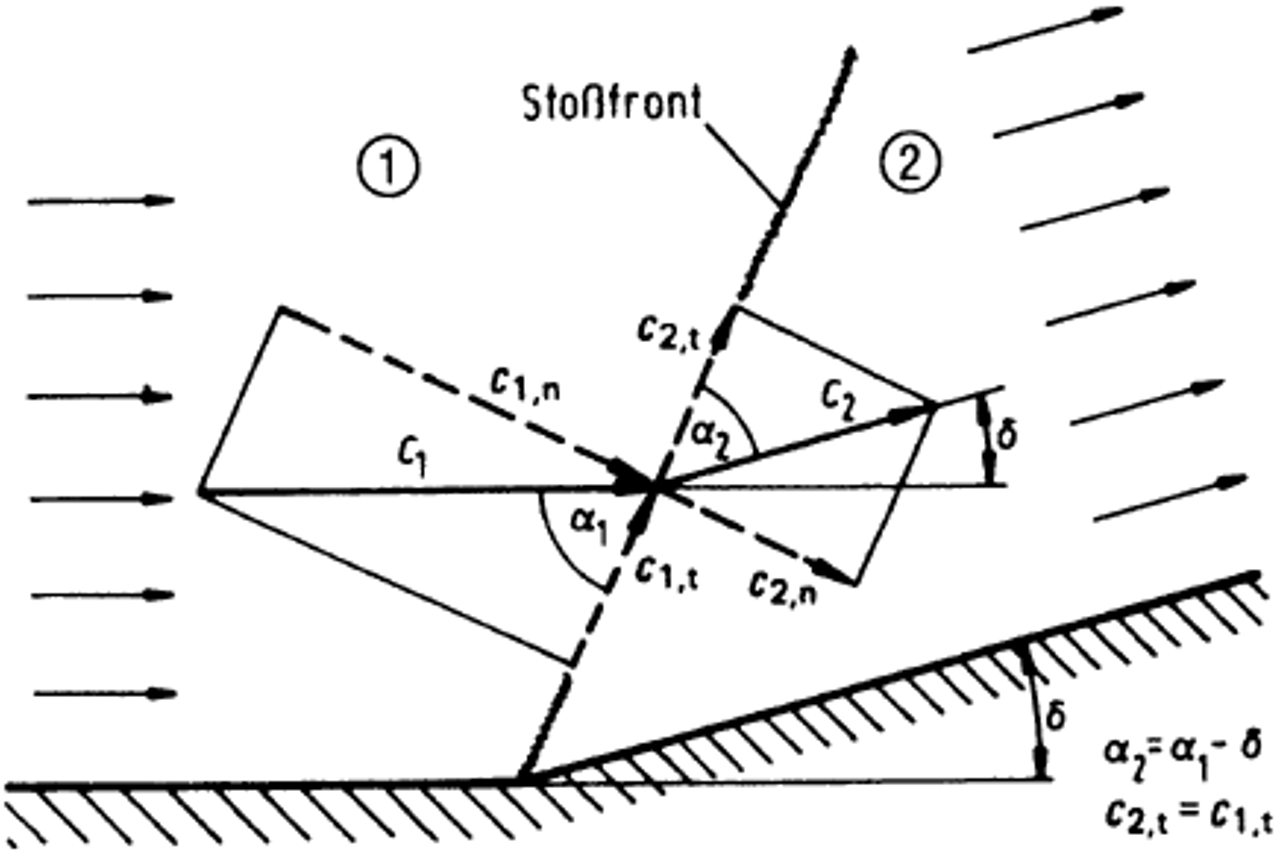
\includegraphics[width=\linewidth]{graphics/Verdichtungsstoss}} \\
		\dfrac{\varrho_2}{\varrho_1} = \dfrac{\tan\alpha_1}{\tan(\alpha_1-\delta)}                                                 &                                                                                             \\
		\dfrac{p_2}{p_1} = 1 + \dfrac{2\ \kappa}{\kappa + 1} \left[\left(\Mach_1\ \sin\alpha_1\right)^2 -1\right]                  &                                                                                             \\
		\cot\delta = \tan\alpha_1 \left[ \dfrac{\kappa+1}{2} \dfrac{\Mach_1^2}{\left(\Mach_1\ \sin\alpha_1\right)^2 -1} -1 \right] & \\
		\text{\quad} &
	\end{array} \]


	% !TeX spellcheck = de_DE
\setcounter{section}{2}

\section{Wärmeübertragung}

\subsection{Wärmestrom und Wärmewiderstände}
	\setlength{\abovedisplayskip}{-20pt}
	\[ \arraycolsep=0.2em  \def\arraystretch{1.8}
	\begin{array}{r l l l l p{1em} l l}
		\Delta T & = R_{ges}\ \dot{Q}                          &                                         &                               &                   &  & R_{ges}        & = \dfrac{1}{k\ A_{wa}}     \\
		R        & = \dfrac{1}{k}                              & = R_{ges}\ A_{wa}                       & = \sum R_{einzel}             & = R_i + R_w + R_a &  & R_w            & = \sum_{N_w}^{j=1} R_{w,j} \\
		\dot{Q}  & = \dfrac{1}{R} A_{wa}\   \Delta T           & = k\ A_{wa}\ \Delta T                   &                               &                   &  & \Delta T       & = T_a - T_i                \\
		\dot{Q}  & = \dfrac{1}{R_i} A_{wa}\ \Delta T_i         & = \alpha_i\ A_{wa}\ \Delta T            &                               &                   &  & \Delta T_i     & = T_{wi} - T_i             \\
		\dot{Q}  & = \dfrac{1}{R_a} A_{wa}\ \Delta T_a         & = \alpha_a\ A_{wa}\ \Delta T            &                               &                   &  & \Delta T_a     & = T_a - T_{wa}             \\
		\dot{Q}  & = \dfrac{1}{R_{w,j}} A_{wa}\ \Delta T_{w,j} &                                         &                               &                   &  & \Delta T_{w,j} & = T_{w,j} - T_{w,j-1}      \\
		\dot{Q}  & = \dot{m}_H\ \abs{\Delta h_H}               & =  \dot{m}_H\ c_{p,H}\ \abs{\Delta T_H} & = \dot{W}_H\ \abs{\Delta T_H} &                   &  & \Delta T_H     & = T_{H2} - T_{H1}          \\
		\dot{Q}  & = \dot{m}_K\ \Delta h_K                     & =  \dot{m}_K\ c_{p,K}\ \Delta T_H       & = \dot{W}_K\ \Delta T_K       &                   &  & \Delta T_K     & = T_{K2} - T_{K1}
	\end{array} \]

\subsection{Ebene Wände -- Platten}
	$ A_{wa} = A_{wi} = A_{wj} = A_{w} = $ konst., Seitenflächen vernachlässigt
		\quad $ R_i = \dfrac{1}{\alpha_i} $
		\quad $ R_{w,j} = \dfrac{\Delta x_j}{\lambda_j} $
		\quad $ R_a = \dfrac{1}{\alpha_a} $

\subsection{Rohr -- Zylinderwände}
	$ A_{wa} = d_a\ \pi\ L $, Deckflächen vernachlässigt
		\qquad $ R_i = \dfrac{d_a}{d_i\ \alpha_i}     $
		\qquad $ R_{w,j} = \dfrac{d_a}{2\ \lambda_j}  \ln\left( \dfrac{d_j}{d_{j-1}} \right) $
		\qquad $ R_a = \dfrac{1}{\alpha_a} $

\subsection{Kugelwände}
	$ A_{wa} = d_a^2\ \pi $
		\qquad $ R_i = \left(\dfrac{d_a}{d_i}\right)^2 \dfrac{1}{\alpha_i} $
		\qquad $ R_{w,j} = \dfrac{d_a^2}{2\ \lambda_j} \left(\dfrac{1}{d_{j-1}} - \dfrac{1}{d_{j}}\right) $
		\qquad $ R_a = \dfrac{1}{\alpha_a} $

\subsection{Parallele Wandschichten}
	$ \dfrac{1}{R_w} = \displaystyle\sum_{N_{w(j)}}^{j=1}   \dfrac{1}{R_{w,j}} $
		\qquad $ \dot{Q} = \dot{Q}_{w,j} =  \displaystyle\sum_{N_{w(j)}}^{j=1}   \dot{Q}_{w,j}$
		\qquad $ R_{w,j} = R_{w,j,seriell}\ \dfrac{A_{wa}}{A_{wa,j}} $

\begin{figure}[h]
	\centering
	\begin{subfigure}{0.24\textwidth}
		\centering
		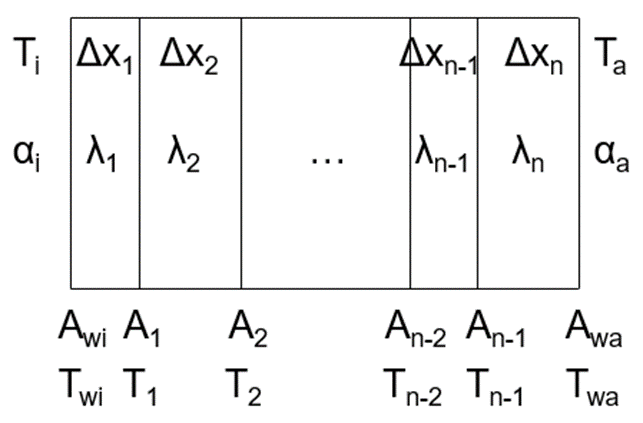
\includegraphics[width=\linewidth]{wand-serie}
		\caption{Serielle Wandschicht}
	\end{subfigure}
	\begin{subfigure}{0.28\textwidth}
		\centering
		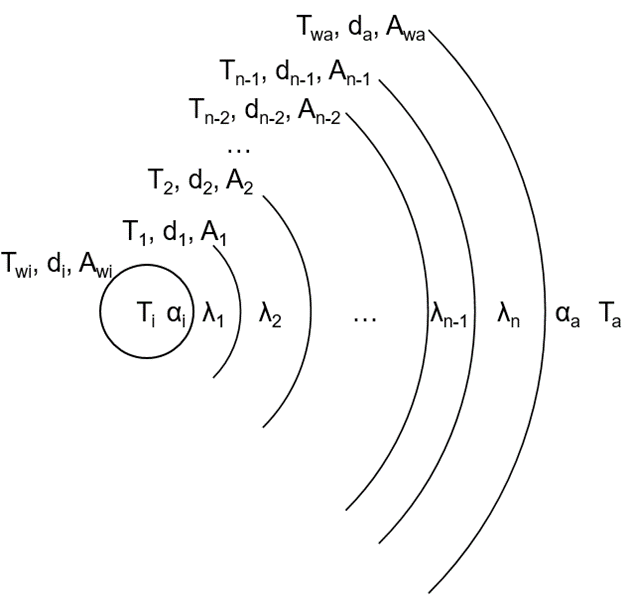
\includegraphics[width=\linewidth]{rohr-serie}
		\caption{Zylinder- und Kugelwand}
	\end{subfigure}
	\begin{subfigure}{0.45\textwidth}
		\centering
		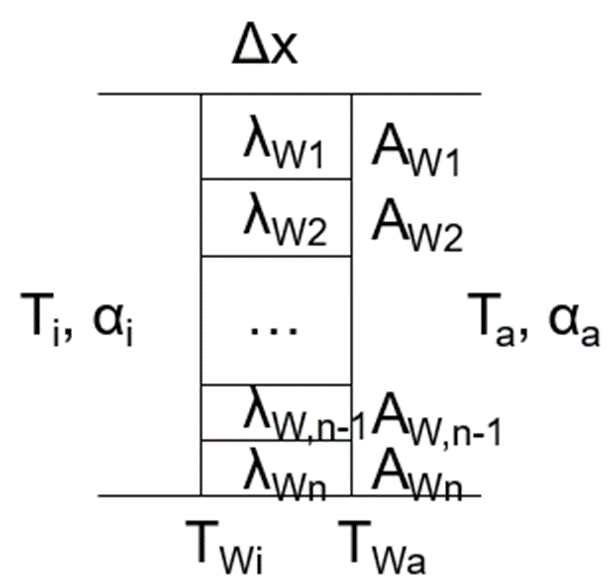
\includegraphics[width=0.4\linewidth]{wand-parallel}
		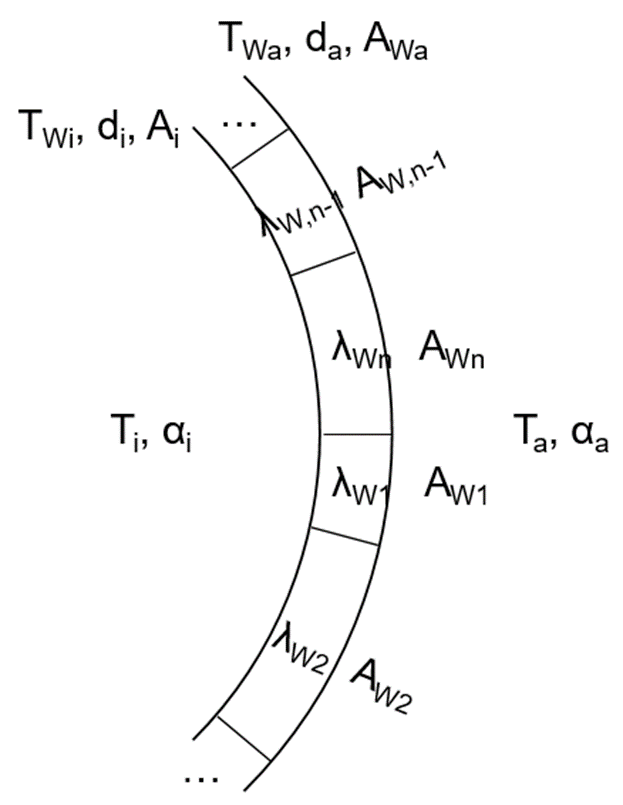
\includegraphics[width=0.5\linewidth]{rohr-parallel}
		\caption{Parallele Wandschichten}
	\end{subfigure}
\end{figure}

\clearpage

\subsection{Rippen}
	$ \eta_{Ri} = \dfrac{\dot{Q}_{Ri}}{\dot{Q}_{Ri,max}} = \dfrac{\tanh(m\ h)}{m\ h} $
		\qquad $ m = \sqrt{\dfrac{\alpha\ U}{\lambda_{Ri}\ A}} $
		\qquad siehe \ref{abb:rippe} (nächste Seite)

	$ \dot{Q}_{Ri} = \lambda_{Ri}\ A_{Ri}\ \Delta T_0\ m \tanh(m\ h) $
		\qquad  $ \Delta T_{(x)} = T_{(x)} - T_u = \Delta T_0\, \dfrac{\cosh\left(m\ h \left(1- \frac{x}{h}\right)\right)}{\cosh(m\ h)} $

	$ \dfrac{A_{w,mit}}{A_{w,ohne}} = 1 - \dfrac{A_{Ri}}{A_{w,ohne}} + \dfrac{A_{w,Ri}}{A_{w,ohne}} $
		\qquad\qquad $ \dfrac{\dot{Q}_{mit}}{\dot{Q}_{ohne}} = \dfrac{\alpha_{mit}}{\alpha_{ohne}} = 1 - \dfrac{A_{Ri}}{A_{w,ohne}}  + \dfrac{U_{Ri}}{A_{w,ohne}} \dfrac{\tanh(m\ h)}{m}$

\subsection{Transiente Wärmeleitung}
	$ a = \dfrac{\lambda}{\varrho\ c_p} $
		\quad $ \Four = \dfrac{a\ t}{s^2} $
		\quad $ \Biot = \dfrac{\alpha\ s}{\lambda} $
		\quad Platten: $ s = \dfrac{\Delta x}{2} $
		\quad Zylinder, Kugeln: $ s = \dfrac{d_a}{a} $
		\quad $\varTheta = \dfrac{T - T_u}{T_0 - T_u}  $

\subsection{Konvektion}
	Durchströmung: $ L_{char} = d_h = \dfrac{4\ A}{U} $ \qquad Umströmung: $ L_{char} = L' = \dfrac{A_w}{U_{proj}}$

	\vskip 3pt
	$ \Reyn = \dfrac{c\ L_{char}}{\nu} = \dfrac{c\ L_{char}\ \varrho}{\mu} $
		\quad $ \Pran = \dfrac{\nu}{a} = \dfrac{\mu\ c_p}{\lambda} = \dfrac{\delta}{\delta_T} $
		\quad $ \Rayl = \dfrac{g\ L_{char}\ \beta\ (T_w - T_{fl})}  {\nu\ a} $
		\quad $ \Nuss = \dfrac{\alpha\ L_{char}}{\lambda} = \dfrac{L_{char}}{\delta_T} $

	\vskip 6pt
	$ \beta_{ideales~Gas} = \dfrac{1}{T_m} $
		\qquad Stoffwerte der WUE bei $ T_m = \dfrac{T_w + T_{fl}}{2} $
		\qquad $ \delta_T = \dfrac{\lambda}{\alpha} $
		\qquad $ \alpha = \dfrac{\lambda}{L'} \Nuss $
		\qquad $ \nu = \dfrac{\mu}{\varrho} $


\subsection{Erzwungene Konvektion}
\subsubsection{Durchströmung}
	\skipabove{-20pt}
	\[ \arraycolsep=0.2em  \def\arraystretch{2}
	\begin{array}{lrll}
		\text{Laminar } \Reyn <2300: & \Nuss_{lam} & \multicolumn{2}{l}{ = \sqrt[3]{3,66^3 + 0,664^3\ \Pran \left(\Reyn \dfrac{d_h}{L}\right)^{\nicefrac{3}{2}}}}\\
		\text{Turbulent } \Reyn>10^4: &\Nuss_{turb} & \multicolumn{2}{l}{ = \dfrac{\nicefrac{ \zeta}{8}\Reyn\Pran}{1 + 12,7 \sqrt{\nicefrac{ \zeta}{8}} \left( \Pran^{\nicefrac{2}{3}} - 1\right)} \ f_1 \ f_2 } \\
		 \zeta = \left(1,8 \log(\Reyn) - 1,5\right)^{-2} & f_1 = 1 + \left(\dfrac{d_h}{L}\right)^{\nicefrac{2}{3}} & \quad f_{2,fl} = \left(\dfrac{\Pran}{\Pran_w}\right)^{0,11} &\quad f_{2,g} = \left(\dfrac{T}{T_w}\right)^{0,45} \\
		\text{Übergang: } \gamma = \dfrac{\Reyn-2300}{10000-2300} &\Nuss & \multicolumn{2}{l}{= (1-\gamma)\cdot \Nuss_{lam,\Reyn=2300} + \gamma\cdot \Nuss_{turb,\Reyn=10000}}\\
		\text{Ringspaltkorrektur: }&\Nuss_{Rs}& = \Nuss\ 0,86 \left(\dfrac{d_{aa}}{d_{ai}}\right)^{0,16}&
	\end{array} \]

\subsubsection{Umströmung}
	\skipabove{-20pt}
	\[ \arraycolsep=0.2em  \def\arraystretch{2}
	\begin{array}{lrrl}
		\text{Keine Anströmung: } & \Reyn<0,1:            & \Nuss_0      & = 0,1\ (\text{Platte}) \quad 0,3\ (\text{Zylinder}) \quad 2\ (\text{Kugel})                        \\
		\text{laminar: }          & 1<\Reyn<10^5:         & \Nuss_{lam}  & = 0,664 \sqrt[3]{\Pran}\sqrt{\Reyn}                                                                \\
		\text{Turbulent: }        & \num{5e5}<\Reyn<10^7: & \Nuss_{turb} & = \dfrac{0,037\ \Reyn^{0,8} \Pran}{1+ 2,443\ \Reyn^{-0,1} \left(\Pran^{\sfrac{2}{3}} - 1\right)} f_3\\
		\multicolumn{2}{c}{f_{3,fl} =\left(\dfrac{\Pran}{\Pran_w}\right)^{0,25}} & \multicolumn{2}{c}{f_{3,g} = \left(\dfrac{T}{T_w}\right)^{0,121}}\\
		\text{Übergang: } & 10<\Reyn<10^7 & \Nuss& = \sqrt{\Nuss_{lam}^2 + \Nuss_{turb}^2}
	\end{array} \]

	\skipabove{-10pt}
	\[ \arraycolsep=1em  \def\arraystretch{1.5}
	\begin{array}{lll}
		\text{Schräg umströmter Zylinder:}
			& \text{Korrekturfaktor } f_5
			& \text{Längs umströmter Zylinder:} \\
		 \Nuss = \Nuss_{Zylinder,\ang{90}} \ f_5
			&  f_5 = \text{siehe Diag. \ref{abb:f5}}
			&  \Nuss =  \Nuss_{Platte}  \left(1+ 2,3 \dfrac{L}{d} \Reyn_L^{-0,5}\right)
	\end{array}\]

\subsubsection{Umströmung in Durchströmung} \label{sec:um-in-durch}
		\skipabove{-20pt}
		\[ \arraycolsep=1em  \def\arraystretch{1.7}
		\begin{array}{ll}
			\text{Hohlraumanteil:}                                                                                                  & \multirow{3}{0.24\textwidth}{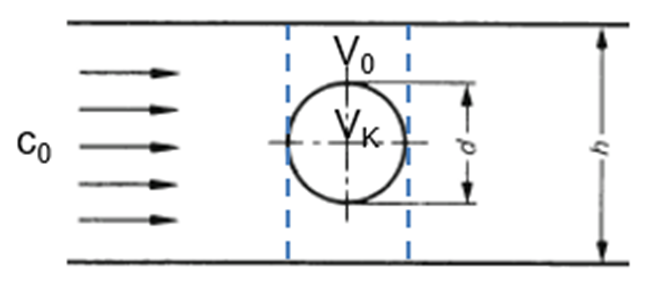
\includegraphics[width=\linewidth]{hohlraumanteil}} \\
			\varepsilon = 1- \dfrac{V_K}{V_0}  \qquad  c = \dfrac{c_0}{\varepsilon}                                                 &                                                                                  \\
			\text{Rohrbündel:}                                                                                                      & \multirow{9}{0.5\textwidth}{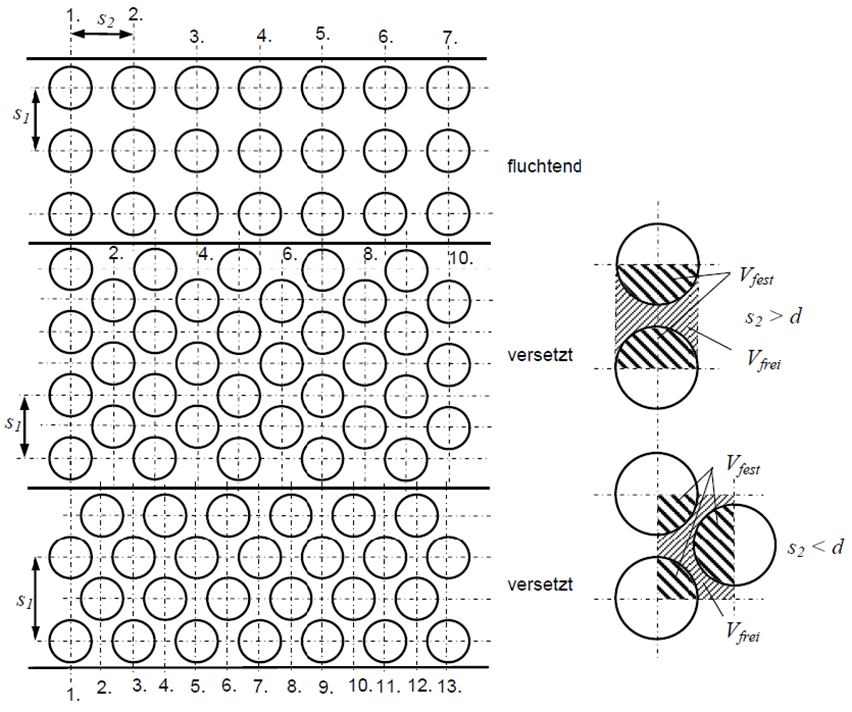
\includegraphics[width=\linewidth]{rohrbuendel}}     \\
			a = \dfrac{s_1}{d}  \qquad  b = \dfrac{s_2}{d}                                                                          &                                                                                  \\
			\Nuss_{B\ue ndel} = \Nuss_{einzel}\ f_A                                                                                 &                                                                                  \\
			f_{A,fluchtend} = 1+ \dfrac{0,7 \left(\nicefrac{b}{a}-0,3\right)}{\varepsilon^{1,5} \left(\nicefrac{b}{a}+0,7\right)^2} &                                                                                  \\
			f_{A,versetzt} = 1 + \dfrac{2}{3\ b}                                                                                    &                                                                                  \\
			n \leq 10:\quad  f_{A,10} = \dfrac{1+ (n-1) f_A}{n}                                                                     &                                                                                  \\
			n \dots \text{Reihen}                                                                                                   &                                                                                  \\
			\null                                                                                                                   &                                                                                  \\
			\null                                                                                                                   &
		\end{array} \]

	\begin{figure}[h]
		\centering
		\begin{subfigure}{7cm}
			\centering
			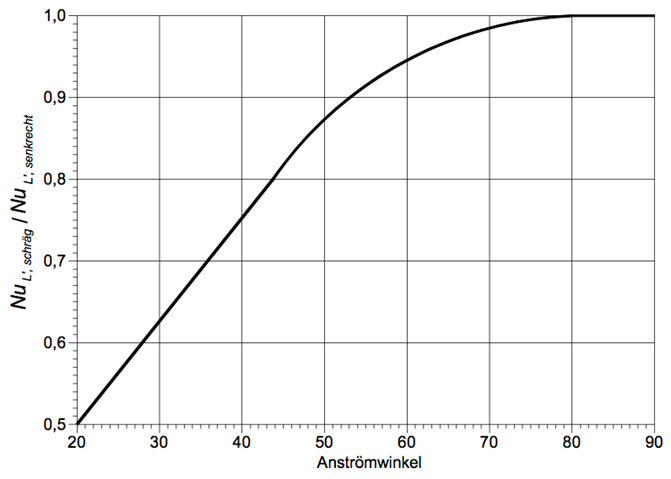
\includegraphics[width=\linewidth]{nusselt-winkel}
			\caption{Weil die Formel für $ f_5 $ noch fehlt}
			\label{abb:f5}
		\end{subfigure}
	\hskip 4em
		\begin{subfigure}{5cm}
			\centering
			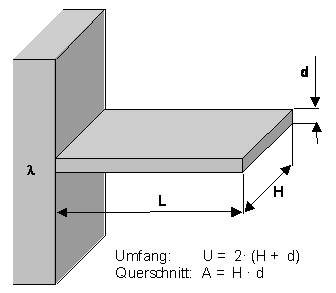
\includegraphics[width=\linewidth]{rippe}
			\caption{Rippengeometrie (für $ m $)}
			\label{abb:rippe}
		\end{subfigure}
		\caption{Hilfen etc.}
	\end{figure}


\clearpage
\subsection{Freie Konvektion}
\subsubsection{Durchströmung}
	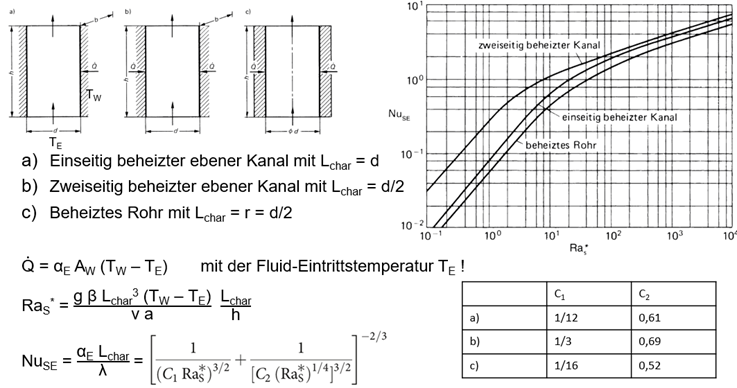
\includegraphics[width=0.9\textwidth]{FK-durchstroemung}

\subsubsection{Umströmung}
	Vertikale Wand: $ \Nuss = (0,825 + 0,387 \Rayl^{\sfrac{1}{6}} \ f_1) $
		\qquad\qquad $ f_1 = (1 + 0,671 \Pran^{\sfrac{-9}{16}}) ^{\sfrac{-8}{27}} $

	\vskip 0.2cm
	Geneigte Wand, Winkel $ \alpha $ zur Vertikalen: \qquad ohne Ablösung: $ \Rayl_{\alpha} = \Rayl\ \cos\alpha $

	\setlength{\abovedisplayskip}{-10pt}
	\[ \arraycolsep=0.7em  \def\arraystretch{1.4}
	\begin{array}{llc}
		\text{mit Ablösung:}
			& \Nuss = 0,56 \displaystyle\sqrt[4]{\Rayl_{krit}\, \cos\alpha} + 0,13 \left( \sqrt[3]{\Rayl} - \sqrt[3]{\Rayl_{krit}} \right)
			& \multirow{8}{5cm}{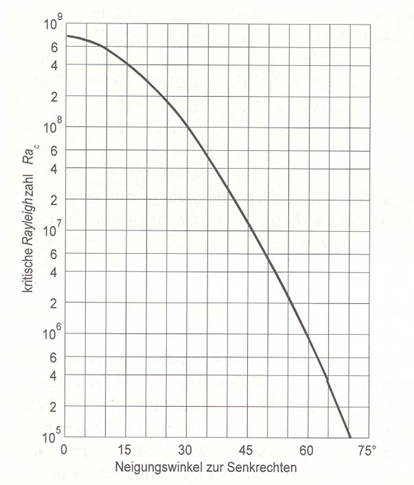
\includegraphics[width=\linewidth]{rayleigh-krit}} \\
		 & \Rayl_{krit} = 10^{(8,9 - 0,013\ \alpha - \num{5,95e-4}\ \alpha^2)} \text{ mit } \alpha \text{ in °} & \\
		 \multicolumn{2}{l}{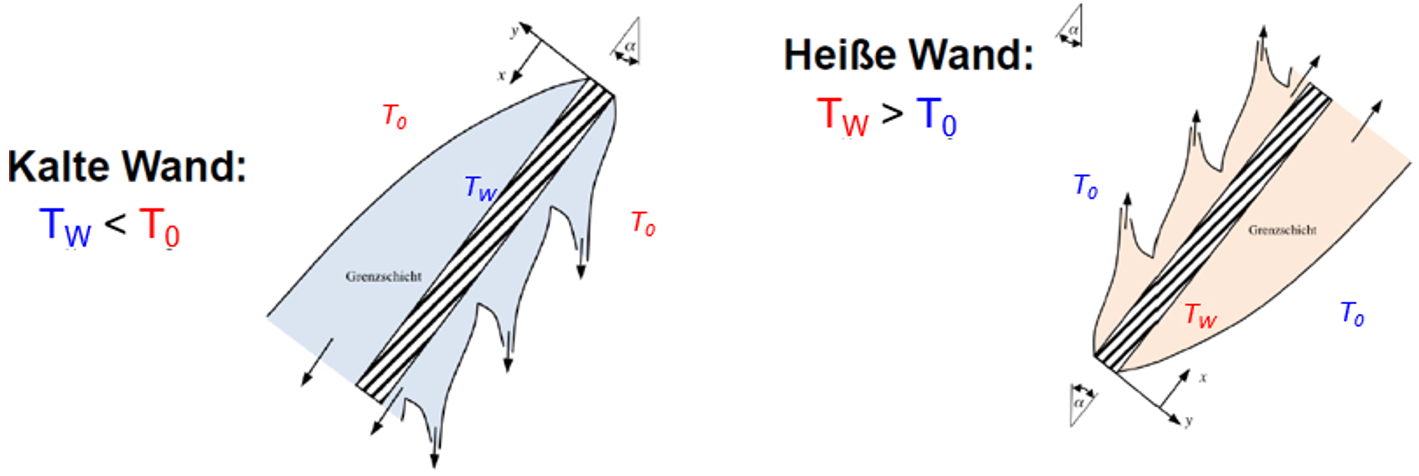
\includegraphics[width=11cm]{wand-abloesung}}
	\end{array}\]

	\setlength{\abovedisplayskip}{-15pt}
	\[ \arraycolsep=0.7em  \def\arraystretch{1.4}
	\begin{array}{lll}
		\text{Horizontale Wand:} &&\\
		 \Rayl\ f_2 \leq \num{7e4}: & \Nuss = 0,766 \displaystyle\sqrt[5]{\Rayl f_2} & f_2 = \left( 1+ 0,536 \Pran ^{\nicefrac{-11}{20}} \right) ^{\nicefrac{-20}{11}} \\
		 \Rayl\ f_2 > \num{7e4}: & \Nuss = 0,15 \displaystyle\sqrt[3]{\Rayl f_2} &\\
		 \text{Horizontaler Zylinder:} & \Nuss = \left(0,752 + 0,387 \sqrt[6]{\Rayl} f_3 \right)^2 & f_3 = \left( 1 + 0,721\Pran^{\nicefrac{-11}{20}}\right) ^{\nicefrac{-8}{27}} \\
		 \text{Kugel:} & \Nuss = 1 + 0,56\, \sqrt[4]{\dfrac{\Pran\Rayl}{0,846 + \Pran}}
	\end{array}\]

\subsubsection{Überlagerung mit erzwungener Konvektion}
	\[ \Nuss = \sqrt[3]{\Nuss_{erzwungen}^3 \pm \Nuss_{frei}^3} \qquad \text{+\dots gleichgerichtete, $-$\dots entgegen-gerichtete Mischkonvektion}\]

% \clearpage
\subsection{Wärmestrahlung zw. Oberflächen}
	\setlength{\abovedisplayskip}{-15pt}
	\[ \arraycolsep=0.4em  \def\arraystretch{1.7}
	\begin{array}{llc}
		\text{Strahlungsbilanz:}                          & a + r + t  =  1                                                                                                                                                                                     & \multirow{12}{2.6cm}{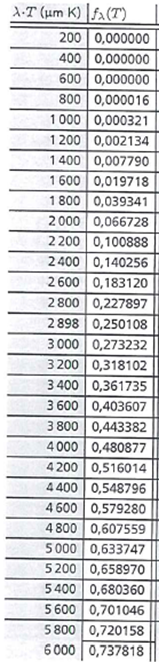
\includegraphics[width=\linewidth]{strahlung-tabelle-1}} \\
		\text{Planck'sches Gesetz:}                       & i_{s(\lambda,T)}  =  \dfrac{\Cone}{\lambda^5\left(\exp\left( \dfrac{\Ctwo}{\lambda\ T} \right) - 1\right)}                                                                                          &                                                                               \\
		\text{Mit: } \Cone=\qty{3,7418e-16}{\W\m\squared} & \Ctwo = \qty{1,438e-2}{\K\m\squared}                                                                                                                                                                &                                                                               \\
		\text{Wien'sches Gesetz:}                         & \lambda_{s,max}  =  \dfrac{2898}{T}  [\unit{\micro\m}]                                                                                                                                              &                                                                               \\
		\text{Stefan Boltzmann Gesetz: mit }\Cs  =  5,67  & \dot{q}_{s(T)}  =  \displaystyle\int_{\lambda = 0}^{\infty} i_{s(\lambda,T)} \ \dd \lambda  =  \Cs \left(\dfrac{T}{100}\right)^4                                                                    &                                                                               \\
		\text{Graue Bande:}                               & \dot{q}_{\lambda,s(T)}  =  \displaystyle\int_{\lambda = 0}^{\lambda} i_{s(\lambda,T)} \ \dd \lambda  = \varepsilon_{(\lambda)}\  f_{(\lambda,T)}\ \dot{q}_{s(T)}                                    &                                                                               \\
		\text{Kirchhoff'sches Gesetz:}                    & a = \varepsilon                                                                                                                                                                                     &                                                                               \\
		\text{Wärmestrom zw. zwei Flächen:}               & \dot{Q}_{12} = C_{12}\ A_{w1}\left[\left(\dfrac{T_1}{100}\right)^4 -\ \left( \dfrac{T_2}{100} \right) ^4\right]                                                                                     &                                                                               \\
		\multicolumn{2}{l}{ \text{Parallele Platten 1 und 2 mit N Platten ($\varepsilon_s$) dazwischen:}}                                                                                                                                                       &                                                                               \\
		\multicolumn{2}{l}{ \qquad C_{12} = \Cs\left[\dfrac{1}{\varepsilon_1} + \dfrac{1}{\varepsilon_2} -1 + N \left(\dfrac{2}{\varepsilon_s} - 1\right)\right] ^{-1}}                                                                                         &                                                                               \\
		\multicolumn{2}{l}{	\text{Konzentrische Zylinder/Kugelschalen (1 innen, 2 außen); N Schalen ($ \varepsilon_s $) dazwischen:}}                                                                                                                           &                                                                               \\
		\multicolumn{2}{l}{	\qquad C_{12} = \Cs\left[ \dfrac{1}{\varepsilon_1} + \dfrac{A_{w1}}{A_{w2}} \left(\dfrac{1}{\varepsilon_2} -1\right) + \left(\dfrac{2}{\varepsilon_s} - 1\right) \displaystyle\sum_{i=1}^{N} \dfrac{A_{w1}}{A_{wsi}} \right] ^{-1}}   & \multirow{12}{2.5cm}{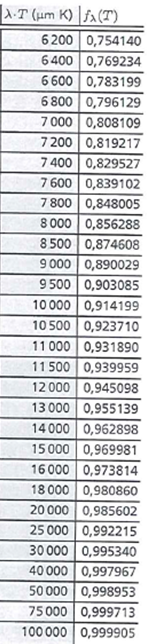
\includegraphics[width=\linewidth]{strahlung-tabelle-2}}     \\
		\text{Beliebig orientierte Flächen:}              & C_{12} = \Cs\dfrac{\varepsilon_1\ \varepsilon_2\ \varphi_{12}}{1-\left(1- \varepsilon_1\right)\left(1-\varepsilon_2\right) \varphi_{12}\ \varphi_{21}\ }                                            &    \\
		\text{\qquad mit Einstrahlzahlen:}                & \varphi_{12} = A_{w2} \dfrac{\cos{\beta_1}\cos{\beta_2}}{r^2\ \pi}   =  \varphi_{21} \dfrac{A_{w2}}{A_{w1}}                                                                                         &                                                                               \\
		\text{Umschlossener Körper 1:}                    & C_{12}  = \Cs \left[ \dfrac{1}{\varepsilon_1} +  \dfrac{A_{w1}}{A_{w2}} \left(\dfrac{1}{\varepsilon_2} - 1\right) \right]^{-1}                                                                      &                                                                               \\
		\text{\qquad wenn }A_{w2} \gg A_{w1}:             & C_{12} = \varepsilon_1\ \Cs                                                                                                                                                                         &                                                                               \\
		\text{Äquivalenter Wärmübergangskoeffizient:}     & \alpha_{Str} = \abs{\dfrac{{\dot{q}}_{Str}}{T_w - T_{fl}}}                                                                                                                                          &                                                                               \\
		\text{Emissionsgrad Umrechnung:}                  & \dfrac{\varepsilon}{\varepsilon_n}                                                                                                                                                                  &                                                                               \\
		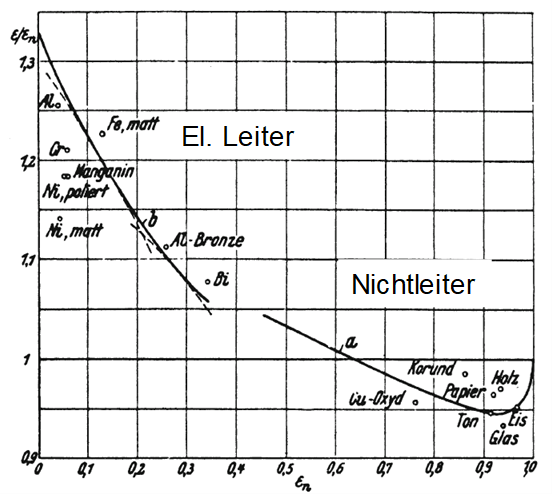
\includegraphics[width=7cm]{strahlung-epsilon}    & 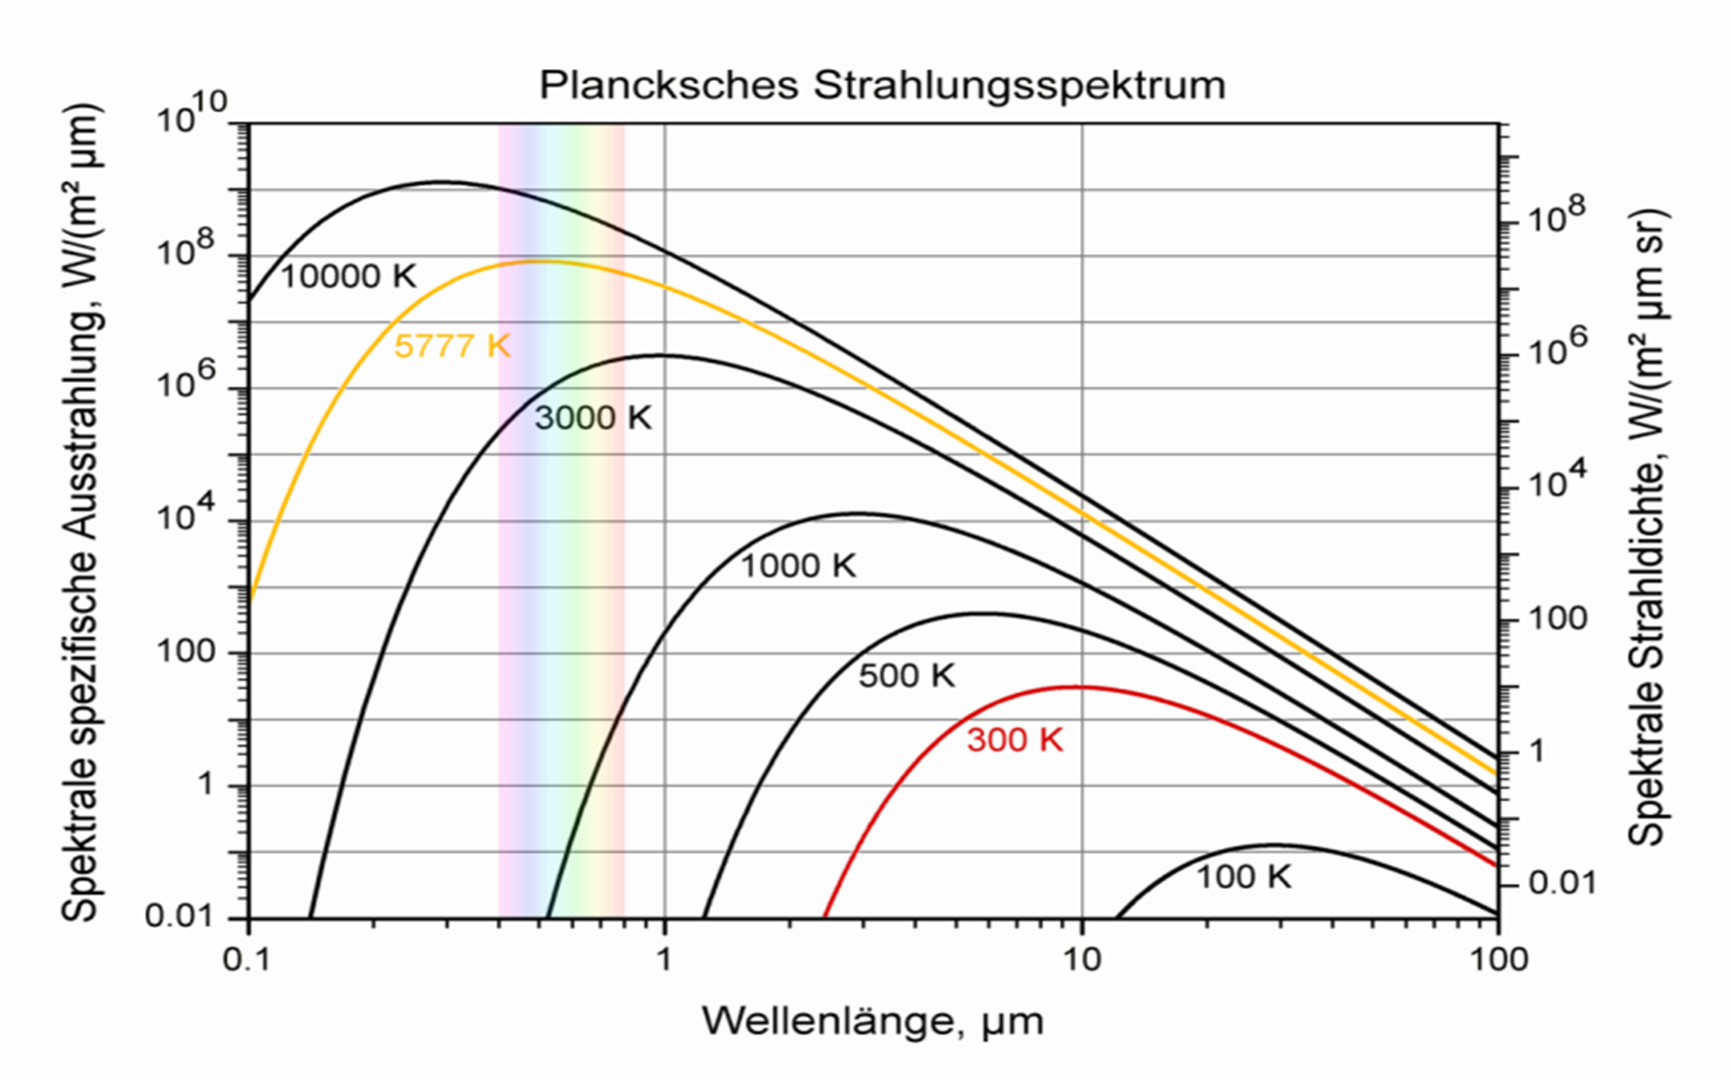
\includegraphics[width=7cm]{strahlung-planck}       &
	\end{array} \]



\subsection{Einseitig konstante Temperatur, Gleichstrom und Gegenstrom}
	\setlength{\abovedisplayskip}{-15pt}
	\[ \arraycolsep=0.4em  \def\arraystretch{1.7}
	\begin{array}{ll}
		\text{Übertragungseinheit}:          & N_i  =  \dfrac{k\ A_{wa}}{{\dot{m}}_i\ {cp}_i}                                                                                                                                                   \\
		\text{Mittlere Temperaturdifferenz:} & \Delta T  =  T_H - T_K  =  \dfrac{\Delta T_a - \Delta T_b} {\ln\left( \dfrac{\Delta T_a}{\Delta T_b}\right)} = \dfrac{\Delta T_b - \Delta T_a} {\ln\left( \dfrac{\Delta T_b}{\Delta T_a}\right)} \\
		\text{Mittlere Wandtemperaturen:}    & T_{wH}  =  T_H - \dfrac{k\ A_{wa}}{\alpha_H\ A_{wH}} \Delta T                                                                                                                                    \\
		                                     & T_{wK}  =  T_K + \dfrac{k\ A_{wa}}{\alpha_K\ A_{wK}} \Delta T
	\end{array} \]

\subsection{Einseitig konstante Temperatur} \label{sec:einseitig-konst-T}
	Übertragungseinheit: \qquad $ N  =  \dfrac{k\ A_{wa}}{\dot{m}\ cp}  =   \ln\left( \dfrac{\Delta T_a}{\Delta T_b} \right)  >  0 $

\subsection{Gleichstrom und Gegenstrom}
	Mittlere Temperaturen:	\qquad	$ T_H \cong \dfrac{T_{H1}+\ T_{H2}}{2}  \qquad T_K\cong \dfrac{T_{K1}+\ T_{K2}}{2} $

\subsection{Vorgangsweise Auslegung}
	\underline{Gegeben:} Geometrie außer Außen-Oberfläche, Einlass-Zustände beidseitig,

		\qquad \textbf{eine Ziel-Auslasstemperatur }

	\underline{Gesucht:} \textbf{Außenoberfläche der wärmeübertragenden Wand},

		\qquad davon abgeleitet Länge oder Rohranzahl etc.

	\begin{singlespace}
	\underline{Berechnung:}
		\begin{enumerate}
		\item Geometrie: Querschnittflächen, char. Abmessungen, etc.
		\item Wärmestrom, andere Auslasstemperatur, mittlere Temperaturdifferenz
		\item Annahme sinnvoller Wandtemperaturen auf beiden Seiten und zw. Wandschichten
		\begin{enumerate}
			\item Bei freier Konvektion, Wärmestrahlung:          \hfill 1. Annahme:	$ T_W \neq T_{fl}  $ \hspace{3cm} \null
			\item In Wärmeübertragern: nur erzwungene Konvektion, \hfill 1. Annahme:	$ T_W = T_{fl} $     \hspace{3cm} \null
		\end{enumerate}
		\item Stoffwerte beidseitig bei Mitteltemperatur zwischen Fluid und Wand
		\item Wand-, heißer -, kalter -, Gesamt-Widerstand, Wärmedurchgangskoeffizient
		\item Außenoberfläche der wärmeübertragenden Wand etc.
		\item Aktualisierung der Wandtemperaturen
		\item Übereinstimmung mit angenommenen Wandtemperaturen?
		\begin{enumerate}
			\item Ja $ \rightarrow $ OK
			\item Nein $ \rightarrow $ zurück zu 4.
		\end{enumerate}
		\end{enumerate}
	\end{singlespace}

\clearpage
\subsection{Vorgangsweise Betriebsnachrechnung}
	\underline{Gegeben:} \textbf{vollständige Geometrie}, Einlass-Zustände beidseitig

	\underline{Gesucht:} \textbf{Auslasstemperaturen beidseitig}

	\begin{singlespace}
		\underline{Berechnung:}
		\begin{enumerate}
			\item Vervollständigung geometrischer Daten (z.B. char. Abmessungen) und der Einlass-Zustände
			\item Annahme von k bzw. Übernahme von k aus Auslegung, iterative Aktualisierung:
		\end{enumerate}
	\end{singlespace}

\subsubsection{Einseitig konstante Temperatur }
	\[ \Delta T_2 = \Delta T_1\ \eul^{-N}   \qquad N\dots \text{ siehe \ref{sec:einseitig-konst-T}} \]

\subsubsection{Gleichstrom}
	\setlength{\abovedisplayshortskip}{-5pt}
	\[
		T_{H2} =  T_{H1} - (T_{H1} - T_{K1})\, \dfrac{\dot{W}_K}{\dot{W}_H + \dot{W}_K} \left(1- \eul^{-\mu\ k\ A_{wa}}\right)
		\hfil \mu = \dfrac{1}{\dot{W}_H} + \dfrac{1}{\dot{W}_K} \hfil
	\]
	\[
		T_{K2} =  T_{K1} - (T_{H1} - T_{K1})\, \dfrac{\dot{W}_K}{\dot{W}_H + \dot{W}_K} \left(1- \eul^{-\mu\ k\ A_{wa}}\right)
	\]

\subsubsection{Gegenstrom}
	\[
		\mu  = \abs{\dfrac{1}{\dot{W}_H} - \dfrac{1}{\dot{W}_K}}
	\]
	\[
		 T_{H2} =  T_{H1} - (T_{H1} - T_{K1})\, \dfrac{1-\ \eul^{-\mu\ k\ A_{wa}}}  {1- \dfrac{\dot{W}_H}{\dot{W}_K}\ \eul^{-\mu\ k\ A_{wa}}}
		 \qquad\qquad
		 T_{K2}  =  {T_{H1}} - (T_{H1} - T_{K1})\, \dfrac{1- \dfrac{\dot{W}_H}{\dot{W}_K}}  {1- \dfrac{\dot{W}_H}{\dot{W}_K}\ \eul^{-\mu\ k\ A_{wa}}}
	\]

\subsection{Rekuperatoren allgemein}
	\[
		P_H = \dfrac{T_{H1} - T_{H2}}{T_{H1} - T_{K1}}
		\qquad\qquad
		P_K = \dfrac{T_{K2} - T_{K1}}{T_{H1} - T_{K1}}
		\qquad\qquad
		\eta = \max(P_H,P_K)
	 \]
	 \[
	 	R_H = \dfrac{\dot{W}_H}{\dot{W}_K} = \dfrac{1}{R_K}
	 	\qquad\qquad
	 	\varTheta = \dfrac{T_H - T_K}{T_{H1} - T_{K1}} = F\ \varTheta_{Gegenstrom}
	 \]

	 $ F $ aus Betriebscharakteristik: $ f(P_H, \,N_H, \,N_K) = 0 $ oder $ f(P_H, \,N_H, \,R_H) = 0 $

\clearpage
\subsection{Regeneratoren}
	\[ \arraycolsep=0.1em  \def\arraystretch{1.6}
	\begin{array}{r l p{3em} r l}
		\Delta Q                                      & = \alpha_H\ A_w  \left(T_H - T_{wH}\right) \Delta t_H  &  & \Delta Q      & = \dfrac{\lambda_s}{\Delta s_w} A_w \left(T_{wH} - T_s\right) \Delta t_H                  \\
		\Delta Q                                      & = \alpha_K\ A_w  \left(T_{wK} - T_K\right) \Delta t_K  &  & \Delta Q      & = \dfrac{\lambda_s}{\Delta s_w} A_w \left(T_s - T_{wK}\right) \Delta t_K                  \\
		\dfrac{\Delta Q}{\Delta t_{H} + \Delta t_{K}} & = \dot{Q} = f\ k_0\ A _{w} \left( T_{H} - T_{K}\right) &  & T_{H} - T_{K} & = \dfrac{\Delta T_{a} - \Delta T_{b}}{\ln \left(\frac{\Delta T_{a}}{\Delta T_{b}}\right)} \\
		\Delta T_{a}                                  & = T_{H1} - T_{K2}                                      &  & \Delta T_{b}  & = T_{H2} - T_{K1} \\
		\dfrac{1}{k_0} & \multicolumn{4}{l}{= \left(\Delta t_{H} + \Delta t_{K}\right)  \left[\dfrac{1}{\alpha_{H}\ \Delta t_{H}} + \dfrac{1}{\alpha_{K}\ \Delta t_{K}} + \dfrac{\Delta s_{W}\ \Phi}{\lambda_{s}}  \left(\dfrac{1}{\Delta t_{H}}+\dfrac{1}{\Delta t_{K}}\right) \right]} \\
		 \text{mit } f,\ \Phi \text{ aus:}
	\end{array}\]


	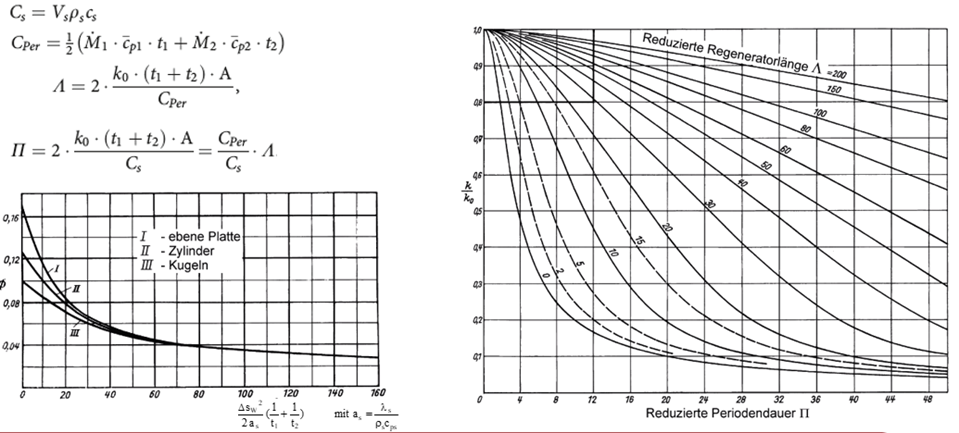
\includegraphics[width=0.95\textwidth]{regeneratoren}
\subsection{Gasstrahlung}
	Wärmestrom zw. heißem Gas (Flamme: $ \varepsilon_g,\ T_g $) einerseits und Wänden ($ T_w,\ \varepsilon_w $)

	und kaltem Gas an Wänden ($ T_w,\ a_g $) andererseits:

	\skipabove{0pt}
	\[ \dot{Q} = \dfrac{\varepsilon_w\ \Cs\ A_w}{1-\left(1-a_g\right)\ (1-\varepsilon_w)\ } \left[ \varepsilon_g \left( \dfrac{T_g}{100} \right)^4 - a_g \left( \dfrac{T_w}{100} \right)^4 \right] \]

	\[ \arraycolsep=0.1em  \def\arraystretch{1.3}
	\begin{array}{r l p{3em} r l}
		\varepsilon_g & = \varepsilon_{\ch{H2O}} + \varepsilon_{\ch{CO2}} - (\Delta\varepsilon)_g                           &  & a_g           & = a_{\ch{H2O}} + a_{\ch{CO2}} - (\Delta \varepsilon)_g                                              \\
		a _{\ch{H2O}} & = \varepsilon_{ \ch{H2O} ( Tw , p \ch{H2O}\ \sfrac{Tg}{Tw})}  \left(\dfrac{T_g}{T_w}\right) ^{0,45} &  & a _{\ch{CO2}} & = \varepsilon_{ \ch{CO2} ( Tw , p \ch{H2O}\ \sfrac{Tg}{Tw})}  \left(\dfrac{T_g}{T_w}\right) ^{0,65}
	\end{array}\]



	Emissionsgrade = Absorptionsgrade aus Diagrammen in Abhängigkeit von Temperatur, Druck, Partialdruck

	von \ch{CO2} bzw. \ch{H2O}, überlappenden Banden und gleichwertiger Schichtdicke $ s $

	\[ s= 0,9\, \dfrac{4\ V_g}{A_w} \]




\end{document}